\def\be{\begin{equation}}
\def\ee{\end{equation}}

\newcommand{\nucl}[3]{ \ensuremath{ \phantom{\ensuremath{^{1}_{#2}}} \llap{\ensuremath{^{#1}}} \llap{\ensuremath{_{\rule{0pt}{.75em}#2}}} \mbox{#3} } }





\documentclass[12pt]{article}
\usepackage{graphicx}
\usepackage{notoccite}
\usepackage{epigraph} % epigraph
\usepackage{float}
\usepackage[hyphens]{url}
\usepackage[square, numbers, comma, sort&compress]{natbib}  % Use the "Natbib" style for the references in the Bibliography
\usepackage{verbatim,listings}  % Needed for the "comment" environment to make LaTeX comments
\usepackage{array}  % Needed for the "comment" environment to make LaTeX comments
\usepackage{vector}  % Allows "\bvec{}" and "\buvec{}" for "blackboard" style bold vectors in maths

% \documentclass[a4paper,12pt]{article}
%\usepackage[a4paper,vmargin={20mm,20mm},hmargin={20mm,20mm}]{geometry}
\usepackage{amsmath,amsfonts,amsthm,color,psfrag,epsf,graphicx}
% \usepackage{pstricks}
\usepackage{enumerate,caption}
%\usepackage[lined,algonl,boxed]{algorithm2e}
\usepackage[ruled,linesnumbered,vlined]{algorithm2e}
\usepackage{float}
% \SpecialCoor
\def\subsum{\mathit{\Sigma}}




\def\ifthesis{\iftrue}
\setcounter{secnumdepth}{2}
\newenvironment{myindentpar}[1]%
{\begin{list}{}%
		{\setlength{\leftmargin}{#1}}%
		\item[]%
	}
	{\end{list}}




\graphicspath{{Figures/}}  % Location of the graphics files (set up for graphics to be in PDF format)
\usepackage{epigraph} % epigraph
%customize: \setlength{\epigraphwidth}{7cm}\setlength{\epigraphrule}{0pt}
%use: \epigraph{text}{reference}

%customize: \setlength{\epigraphwidth}{7cm}\setlength{\epigraphrule}{0pt}
%use: \epigraph{text}{reference}
\begin{document}
\bibliographystyle{unsrt}
 
\section{Introduction}
%Langmuir probes are a powerful diagnostic, providing measurements of the plasma potential ($V_{p}$), electron density ($n_e$) and temperature ($T_e$) in the scrape-off layer of tokamak experiments \cite{Stangeby}. Accurate measurements of these quantities are necessary in order to model various divertor phenomena such as recycling and detachment 

Langmuir probes are built into divertor plates such that their surface is flush with the surface of the divertor tiles. Probes in this configuration are known as flush-mounted probes (FMP). These tiles and the FMPs, are capable of surviving the high power flux of the SOL, if the magnetic field meets the tiles at a grazing angle of incidence, as this spreads the flux over a larger area, reducing the thermal load on the probe surface. As has been discussed previously in Chapter 2, interpretation of Langmuir probe measurements in strongly magnetised plasma is complicated by the influence of the magnetic field on charged particle collection \cite{Stangeby}. In a strong magnetic field, the collection area of the probe ($A_{eff}$), is reduced from the surface area of the probe ($A$) to the projected area of the probe along the field ($A_{eff} = A sin(\theta)$), where $\theta$ is the angle between the magnetic field and the probe surface. For a standard Langmuir probe inserted into a plasma, $A_{eff}$ is relatively easy to calculate. A measurement of the ion saturation current and the electron temperature can then be used to determine the electron density, as can be seen in equation \ref{eq:isat}
\be 
I_{sat} = n_e e A_{eff} c_s
\label{eq:isat}
\ee

Due to the grazing angle of incidence the magnetic field makes with the divertor tiles, the FMP configuration provides further complications to the interpretation of the measurements. At grazing angles of incidence, the effective collection area of the probe is reduced significantly and can be comparable to the area of the sheath in front of the probe. The Child-Langmuir law, equation \ref{eq:CL}, states that the thickness of the sheath ($s$) in front of the probe depends on the bias voltage ($V_B$), increasing as the probe is biased more negatively relative to the surrounding tiles \cite{child}, \cite{childL}. 
\be
s \propto \lambda_D {\left(\frac{e V_B}{T_e}\right)}^\frac{3}{4}
\label{eq:CL}
\ee

Ions that enter the sheath are drawn to the probe by the strong electric fields present in this region. With increasingly negative bias voltage, the sheath size expands and so does the effective collection area of the probe. As a result, current-voltage (I-V) characteristics obtained from FMPs deviate from the well known ideal characteristics derived from the one-dimensional model presented in Chapter 2, with non-saturation of the ion current often observed \cite{Gunn-1995}. An example of an I-V curve obtained by a FMP is shown in figure \ref{fig:non-sat}. Standard probe theory cannot be used to interpret FMP measurements \cite{FMP_tilt}.   Applying the standard analysis procedure to FMP data yields temperatures and densities that are too high \cite{tilting}, as the non-saturation of the ion current at highly negative voltages is interpreted as a still present, but declining electron current by the fitting algorithm. In order for FMP measurements to return the correct values for the plasma parameters, the effective collection area of the probe must be known. 

 
\begin{figure}[H]
\centering
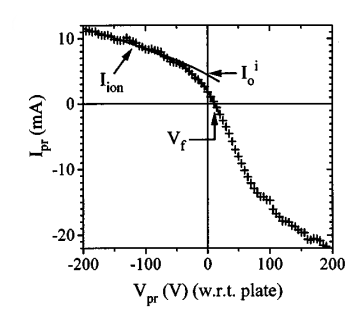
\includegraphics[width=0.9\textwidth]{non_sat.png}
\caption{A FMP I-V characteristic, taken from \cite{gunn_magnetisation}.}
\label{fig:non-sat}
\end{figure}



\section{Overview of FMP theory}
It is clear for FMPs that the area of the sheath cannot be neglected, as it often is for probes in the standard configuration. The effective area for a FMP consists of the geometrical projection of the surface area of the probe and the area of the sheath in front of the probe, which will increase with voltage applied to the probe
\be 
A_{eff} = A \sin{\theta} + A_{sheath}
\ee 
This assumes that due to the strong electric fields present in the sheath, any ions that enter the sheath will be collected by the probe.

 Models of ion collection by FMPs have been developed that take into account the increasing size of the sheath as the probe is biased more negatively. Early modelling attempts included a non-linear term to account for the Child-Langmuir expansion, obtaining an equation for $A_{sheath}$ of the form
\be 
A_{sheath} = w \times s = w k \lambda_D {\left(\frac{e V_B}{T_e}\right)}^\frac{3}{4}
\ee 
Here, $w$ is the width of the sheath, which is taken to be the probe width, $s$ is the sheath thickness and $k$ is the constant of proportionality in the Child-Langmuir law. The new value for $A_{eff}$ is then substituted into equation \ref{eq:isat}, obtaining a new equation that could then be fitted to the slope of the ion current to extract the plasma parameters.

These early models correctly predicted that the sheath in front of the probe would be larger than the sheath in front of the floating tiles either side of it, however, they neglected both the complex structure of the transition region between a plasma and a material surface in a magnetised plasma and the exact trajectories of ions moving through these transitional layers.  As discussed in Chapter 2, the transition region in a magnetised plasma consists of three layers, the quasi-neutral pre-sheath, the magnetic pre-sheath (MPS) and the Debye sheath (DS). Ions enter the MPS with parallel velocity along the field lines exceeding the Bohm speed and exit the MPS with speeds normal to the surface exceeding the Bohm speed. From current continuity the following equation is obtained \cite{current-con}
\be 
n_{mps} \ c_s \sin{\theta} = n_{ds} \ c_s 
\label{eq:current-con}
\ee 
Where $n_{mps}$ and $n_{ds}$ are the densities at the entrance to the MPS and DS respectively. It can be seen from equation \ref{eq:current-con} that the density at 
the entrance to the DS is significantly lower than that at the MPS entrance for grazing angles of incidence. As a result of this density drop, the thickness of the sheath, which scales with Debye length, in front of the probe and the floating wall can be greatly enhanced compared to the unmagnetised case.
 

An analytical fluid model that incorporated the MPS density drop was developed by Weinlich and Carlson in order to understand the lack of saturation of the ion current \cite{asdex_FMP}. This model also considers the trajectories of ions as they move through the MPS and DS. In the Weinlich and Carlson model, the probe sheath was considered to be a rectangular, sharp edged box. Any ion that enters the sheath is drawn to the probe. The model of the sheath is shown in figure \ref{fig:wc-sheath}. The probe has a length $L$ and a width $w$ extending into the plane. The probe is biased negatively with respect to the floating wall around it and so the thickness of the DS in front of the probe is enhanced relative to the DS in front of the wall by an amount $s$. Ions travel parallel to the field lines until they enter the MPS, at which point they begin to follow a curved trajectory until attaining a velocity normal to the wall which satisfies the Bohm Criterion on entry to the DS. For ions that enter the MPS at the same speed, all trajectories in the MPS will be equal in length and shape, regardless of whether ions reach the wall's DS or the probe's. As the probe has a thicker DS, the entrance of the probe's MPS will be shifted upstream. This is illustrated in figure \ref{fig:wc-sheath}, where the entrance to the MPS is represented by the dashed lines, corresponding to an upstream image of the DS. 

The trajectories, lines 1 and 2, drawn with bold lines, mark the boundaries between ions that make it to the probe and those that hit the wall. Ions following a trajectory in between lines 1 and 2, exit the MPS at the entrance to the probe's DS and hit the probe.  Circled on line 2 is a bifurcation point in the trajectory. An ion following a trajectory just outside of line 2 will travel parallel to the field, past the bifurcation point, only turning towards the normal once reaching the MPS entrance of the wall, shown in dashed lines, which is the same fixed distance from the wall's DS as the distance between the MPS and DS of the probe. Therefore, there exists a region of the wall, between the two bifurcated trajectories, that the ions cannot access. A lower current is expected in this region. At the leading edge of the probe, located above line 1 by an amount $s$ at the MPS entrance, is another ion trajectory. This represents ions that would reach the probe due to its projected length, ($L \sin \theta$), the enhanced thickness of the probe's DS is not relevant to these ions. However, for ions between this trajectory and line 1, the increased sheath thickness allows these ions to reach the probe's DS. Without the sheath enhancement, these ions would hit the wall instead. All ions following trajectories in this region, arrive in the probes DS at the same horizontal position above the probe. The model therefore predicts a focusing effect and hence, an enhancement of the ion current on the leading edge of the probe.
\begin{figure}[H]
\centering
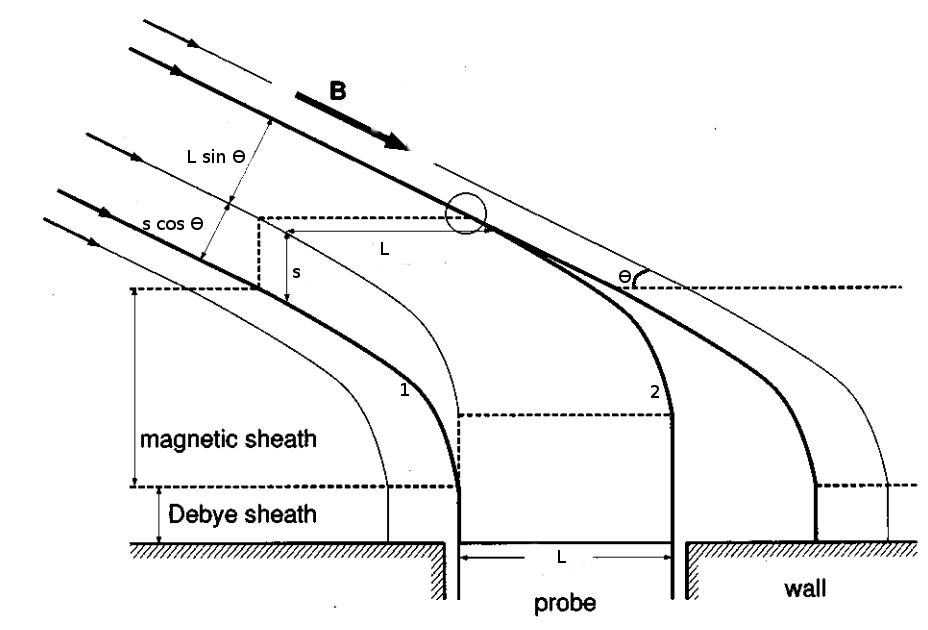
\includegraphics[width=0.9\textwidth]{wc_sheath.png}
\caption{Model of the sheath in front of a FMP. Taken from \cite{asdex_FMP}.}
\label{fig:wc-sheath}
\end{figure}

This model does not take into account effects of the finite gyroradius of the ions. In order to capture these effects a kinetic treatment of the ions is required. Detailed, two-dimensional particle-in-cell (PIC) simulations of small FMPs in plasmas with oblique magnetic fields were carried out by Bergmann \cite{bergmann_1994}. The fluid model's predictions of an enhanced ion current to the leading edge of the probe and a depleted current to the wall beyond the trailing edge of the probe were observed in the PIC simulations. The work detailed in \cite{bergmann_1994} and \cite{Bergmann-2002} is the foundation of the results presented in this chapter, it is therefore necessary to summarise this work before proceeding to the results.

\section{Summary of Previous Particle-In-Cell Simulations of Flush-Mounted Probes}

In \cite{bergmann_1994}, the motion of ions and electrons were tracked as they followed magnetic field lines towards an absorbing surface, consisting of a floating wall and a probe that was biased negatively with respect to the floating potential. The simulation domain is shown in figure \ref{fig:bergmann_sim_model}. Both ions and electrons are treated kinetically although a guiding centre approximation for the electrons was used to speed up the simulations.

\begin{figure}[H]
\centering
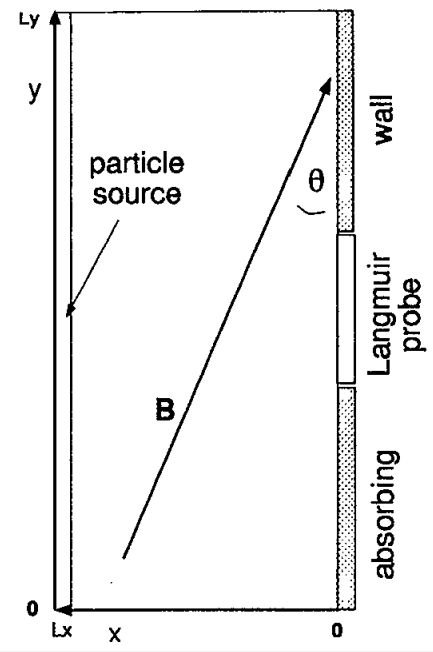
\includegraphics[width=5cm, height = 7cm]{Bergmann_model.png}
\caption{A representation of the particle-in-cell simulation domain used to model the particle collection of FMPs. Taken from \cite{Bergmann-1994}.}
\label{fig:bergmann_sim_model}
\end{figure}

As with experimental data, the ion current in the PIC simulations was found not to saturate at highly negative voltages. A sheath that scaled with voltage was found to be responsible for this non-saturation. It was found that the sheath thickness in front of the probe ($\Delta$) was described by the following relation
\be 
\Delta  = \Delta_0 + \Delta_1 {\left| V \right|}^{3/4}
\ee
Where $V$ is the bias voltage applied to the probe, relative to the floating wall.
\be 
V = \frac{V_{wall}-V_{probe}}{T_e}
\ee 
$\Delta_0$ is the thickness of the sheath in front of the probe when it is at the floating potential. $\Delta_1$ is a coefficient that takes into account the enhanced thickness of the Debye sheath when the probe is biased more negatively than the surrounding wall.  It was found that $\Delta_0$ decreases as $\theta \to 0$, despite the MPS density drop having a larger effect at low angles. For decreasing $\theta$, more of the potential drop is contained in the MPS rather than the DS. As there is less of a potential drop across the DS, the thickness of the DS is reduced. This effect more than makes up for the enhanced Debye length. $\Delta_1$, on the other hand, increases as $\theta \to 0$. It was found that 
\be 
\Delta_1 \approx \frac{0.5 \lambda_D}{\sqrt{\sin \theta}}
\ee
The ion focusing effect is more powerful at smaller angles. When the probe is floating, so at the same potential as the surrounding tiles, $V = 0$ and therefore, the sheath thickness in front of the probe is the same as that of the sheath in front of the floating wall ($\Delta = \Delta_0$). As a result, no ion focusing effects are observed, the probe collects a current $I_0$, which is the current travelling along the flux tube subtended by the probe 
\be 
I_0 = e n_e c_s L sin \theta 
\ee 
Where $n_e$ is the electron density at the entrance to the MPS. Here the sound speed is $c_s = \sqrt{(T_e + \gamma_i T_i)/m_i}$. $\gamma_i$ is the adiabatic index determined by the number of effective degrees of freedom for the ions (f), $\gamma_i =(f+2)/f$. At grazing angles of incidence, f = 2. For a standard Langmuir probe, where the collection area of the probe is much greater than the sheath area, the sheath area is negligible. As a result, $I_0$ would be a good approximation for the ion current at all negative voltages up to the plasma potential. This isn't the case for a FMP, where the sheath area is comparable to the effective collection area of the probe. The current to the simulated probes was well described by the following equation 
\be 
I/I_0 = 1 + a {\left|V\right|}^{3/4} -e^V
\label{eq:IV}
\ee
The parameter \textit{a} is directly proportional to $\Delta_1$. In \cite{bergmann_1994} paper, a value for \textit{a} was derived 
\be 
a = \left( 0.5 + 0.4\frac{1 - \sin \theta}{\sin \theta}\right) \frac{1}{L\sqrt{sin\theta}}
\ee
However, this derivation used a more complicated sheath model than that presented in figure \ref{fig:wc-sheath}. Due to computational demands, simulations in \cite{bergmann_1994} were carried out for small probes, where the ratio of probe length to ion gyroradius was smaller than that in experiments. The complicated model presented in \cite{bergmann_1994} was found to be a good approximation for small probes. The model was later extended to larger probes with realistic ratios of probe length to ion gyroradius \cite{Bergmann-2002}.  For these larger probes, the rectangular approximation of the sheath was found to be a better representation. For this model, a new sheath expansion parameter was derived
\begin{equation}
a = \frac{c_1 + c_2 \cot{\theta}}{{\sin^{1/2}{\theta}}} \frac{\lambda_D}{L}
\label{eq:sheath_expansion}
\end{equation}
The probe sheath expands both in thickness away from the wall and laterally along the length of the wall. $c_1$ is a coefficient that describes the lateral sheath expansion while $c_2$ is related to the increased sheath thickness in front of the probe. By plotting $a L \sin^{1/2}{\theta}$ against $\cot {\theta}$ it is possible to measure $c_1$ and $c_2$. It was found that $c_1 =0.5$ and $c_2$ depended on the probe length relative to $\lambda_D$, reaching a maximum value of 0.6 once $L \approx 400 \lambda_D$. This model was found to explain measurements of the non-saturation of the ion current on ASDEX-Upgrade \cite{Bergmann-2002}.

In an experiment, there is always a gap between the FMP and the surrounding divertor tiles. The gap exposes the leading side of the probe to plasma and so could increase the effective collection area of the probe. The model in \cite{Bergmann-2002} does not take into account the gap. This may not be an issue for the FMPs of ASDEX-Upgrade as the probes deployed measure 5 by 40 mm with the largest side orientated parallel to the magnetic field lines \cite{asdex_FMP} and so the additional current reaching the side of the probe may be negligible. However, the MAST probes are much smaller, with dimensions 2 by 5 mm and a significant probe gap of 1 mm. If there is an additional current to the side of the probe, this would need to be taken into account to extract an accurate plasma density from the measured ion current. To investigate the effects of the probe-tile gap, PIC simulations were carried out with VSim. The remainder of this chapter introduces the simulation model and presents the results of the simulations. 


 %This gave good agreement with experimental data obtained on ASDEX Upgrade a These simulations were extended by Bergmann to include larger probes with realistic probe length to ion gyroradius ($\rho_i$) \cite{Bergmann-2002}. Bergmann found the sheath in front of a FMP increases in thickness both vertically and laterally as the probe bias becomes more negative. In the simulations, the non-saturation of the ion current was well described by a sheath expansion parameter ($a$) that takes into account the magnetic presheath (MPS) density drop and varies as a function of $\theta$.




%Result from second paper 
%Introduce, his sheath model,  sheath expansion parameter and the IV curve fitting 
%Maybe summarise the ExB stuff 
%
%Lacks the gap 
%
%
%As bergmann most thorough, resolve finite gyroradius effects etc, carried on with this model incorporating gaps
\section{The Simulation Model}
%Focus on we allow it to float naturally and this will be compared in section to show the no gap model to Bergmanns to show key results

The simulation model has two spatial dimensions and three velocity components (2D3V). A plasma consisting of singly charged ions and electrons is studied. The full gyromotion of electrons and ions is tracked as they move in a self-consistent electric field and a prescribed, homogeneous magnetic field. The domain captures the entire probe length with the probe located at the centre of the domain surrounded by a floating wall. The simulations model a region of plasma above the probe of width 5 $\rho_i$ to capture the MPS. An additional buffer region of width 1 $\rho_i$ is added to the particle source region. The electric field in this region is zero, this allows particles with velocity parallel to the magnetic field ($v_{\parallel}$),  directed towards the probe-wall interface to complete their gyromotion around the magnetic field without being deleted from the simulation. Particles that are moving away from the probe (with negative $v_{\parallel}$) that enter this region, travel to the beginning of the domain and are removed from the simulation. A two dimensional slab model of the simulation domain is presented in figure \ref{fig:2D_domain}. 


The y axis is treated periodically. Particles follow field lines towards the probe-wall interface. Particles that reach the interface are removed from the simulation. Those that hit the floating wall deposit their charge there allowing a charge density and electrostatic potential to evolve naturally, to a steady state without imposing additional boundary conditions on the walls. The domain is initially filled with a spatially uniform Maxwellian plasma. Particles are injected into the simulation domain at the source region to replenish those lost to the probe and walls. The parallel component of velocity for the particles is sampled from the Emmert distribution \cite{Emmert} as this conserves the plasma temperature in the domain. The two perpendicular velocity components are sampled from a Maxwellian distribution. The potential at the beginning of the domain is set to 0 V and the probe potential is fixed to $V_{probe}$, the wall evolves to a floating potential ($V_f$).   

The domain is a rectangle in the x-y plane and models the toroidal length of the probe which lies along the y axis. The plasma is assumed to be uniform along the ignored z-axis. The domain has lengths $L_x$ and $L_y$ respectively and the probe has length $L$. The magnetic field is inclined to the wall by an angle $\theta$ where  $\tan(\theta) = B_x/B_y$. In these simulations the field is directed in the toroidal direction, along the largest dimension of the probe, there is no poloidal component.

A reduced ion mass ($m_i$) was used in the simulations equivalent to 900 $m_e$, where $m_e$ is the electron mass. The reduced ion mass decreases $\rho_i$ which in turn decreases the required length of the simulation domain in the x direction. It also increases the ion sound speed thus reducing the time for the simulation to reach steady state. Simulations were carried out with the same probe length to ion gyroradius ratio as in the MAST divertor region, as the simulated gyroradius is less than in experiments, the length of the simulated probe is therefore shorter than in experiments too. The ion gyroradius to Debye length ($\lambda_D$) ratio from experiments was also conserved in the simulations. For a typical shot on MAST, the ion gyroradius in the MAST divertor is estimated to be $0.9$ mm, but in the simulation, with less massive ions, this is reduced to $0.42$ mm. The probe length in the simulations is then reduced from $5$ mm to $2.38$ mm. The Debye length is also reduced, requiring a small increase in density to conserve the ratio. The simulated densities are still well within the range of values seen in the MAST divertor. Typical simulation parameters are given in table \ref{tab:sim_parameters}. The results presented will be for these simulation parameters unless otherwise stated.
\begin{figure}[H]
	\centering
	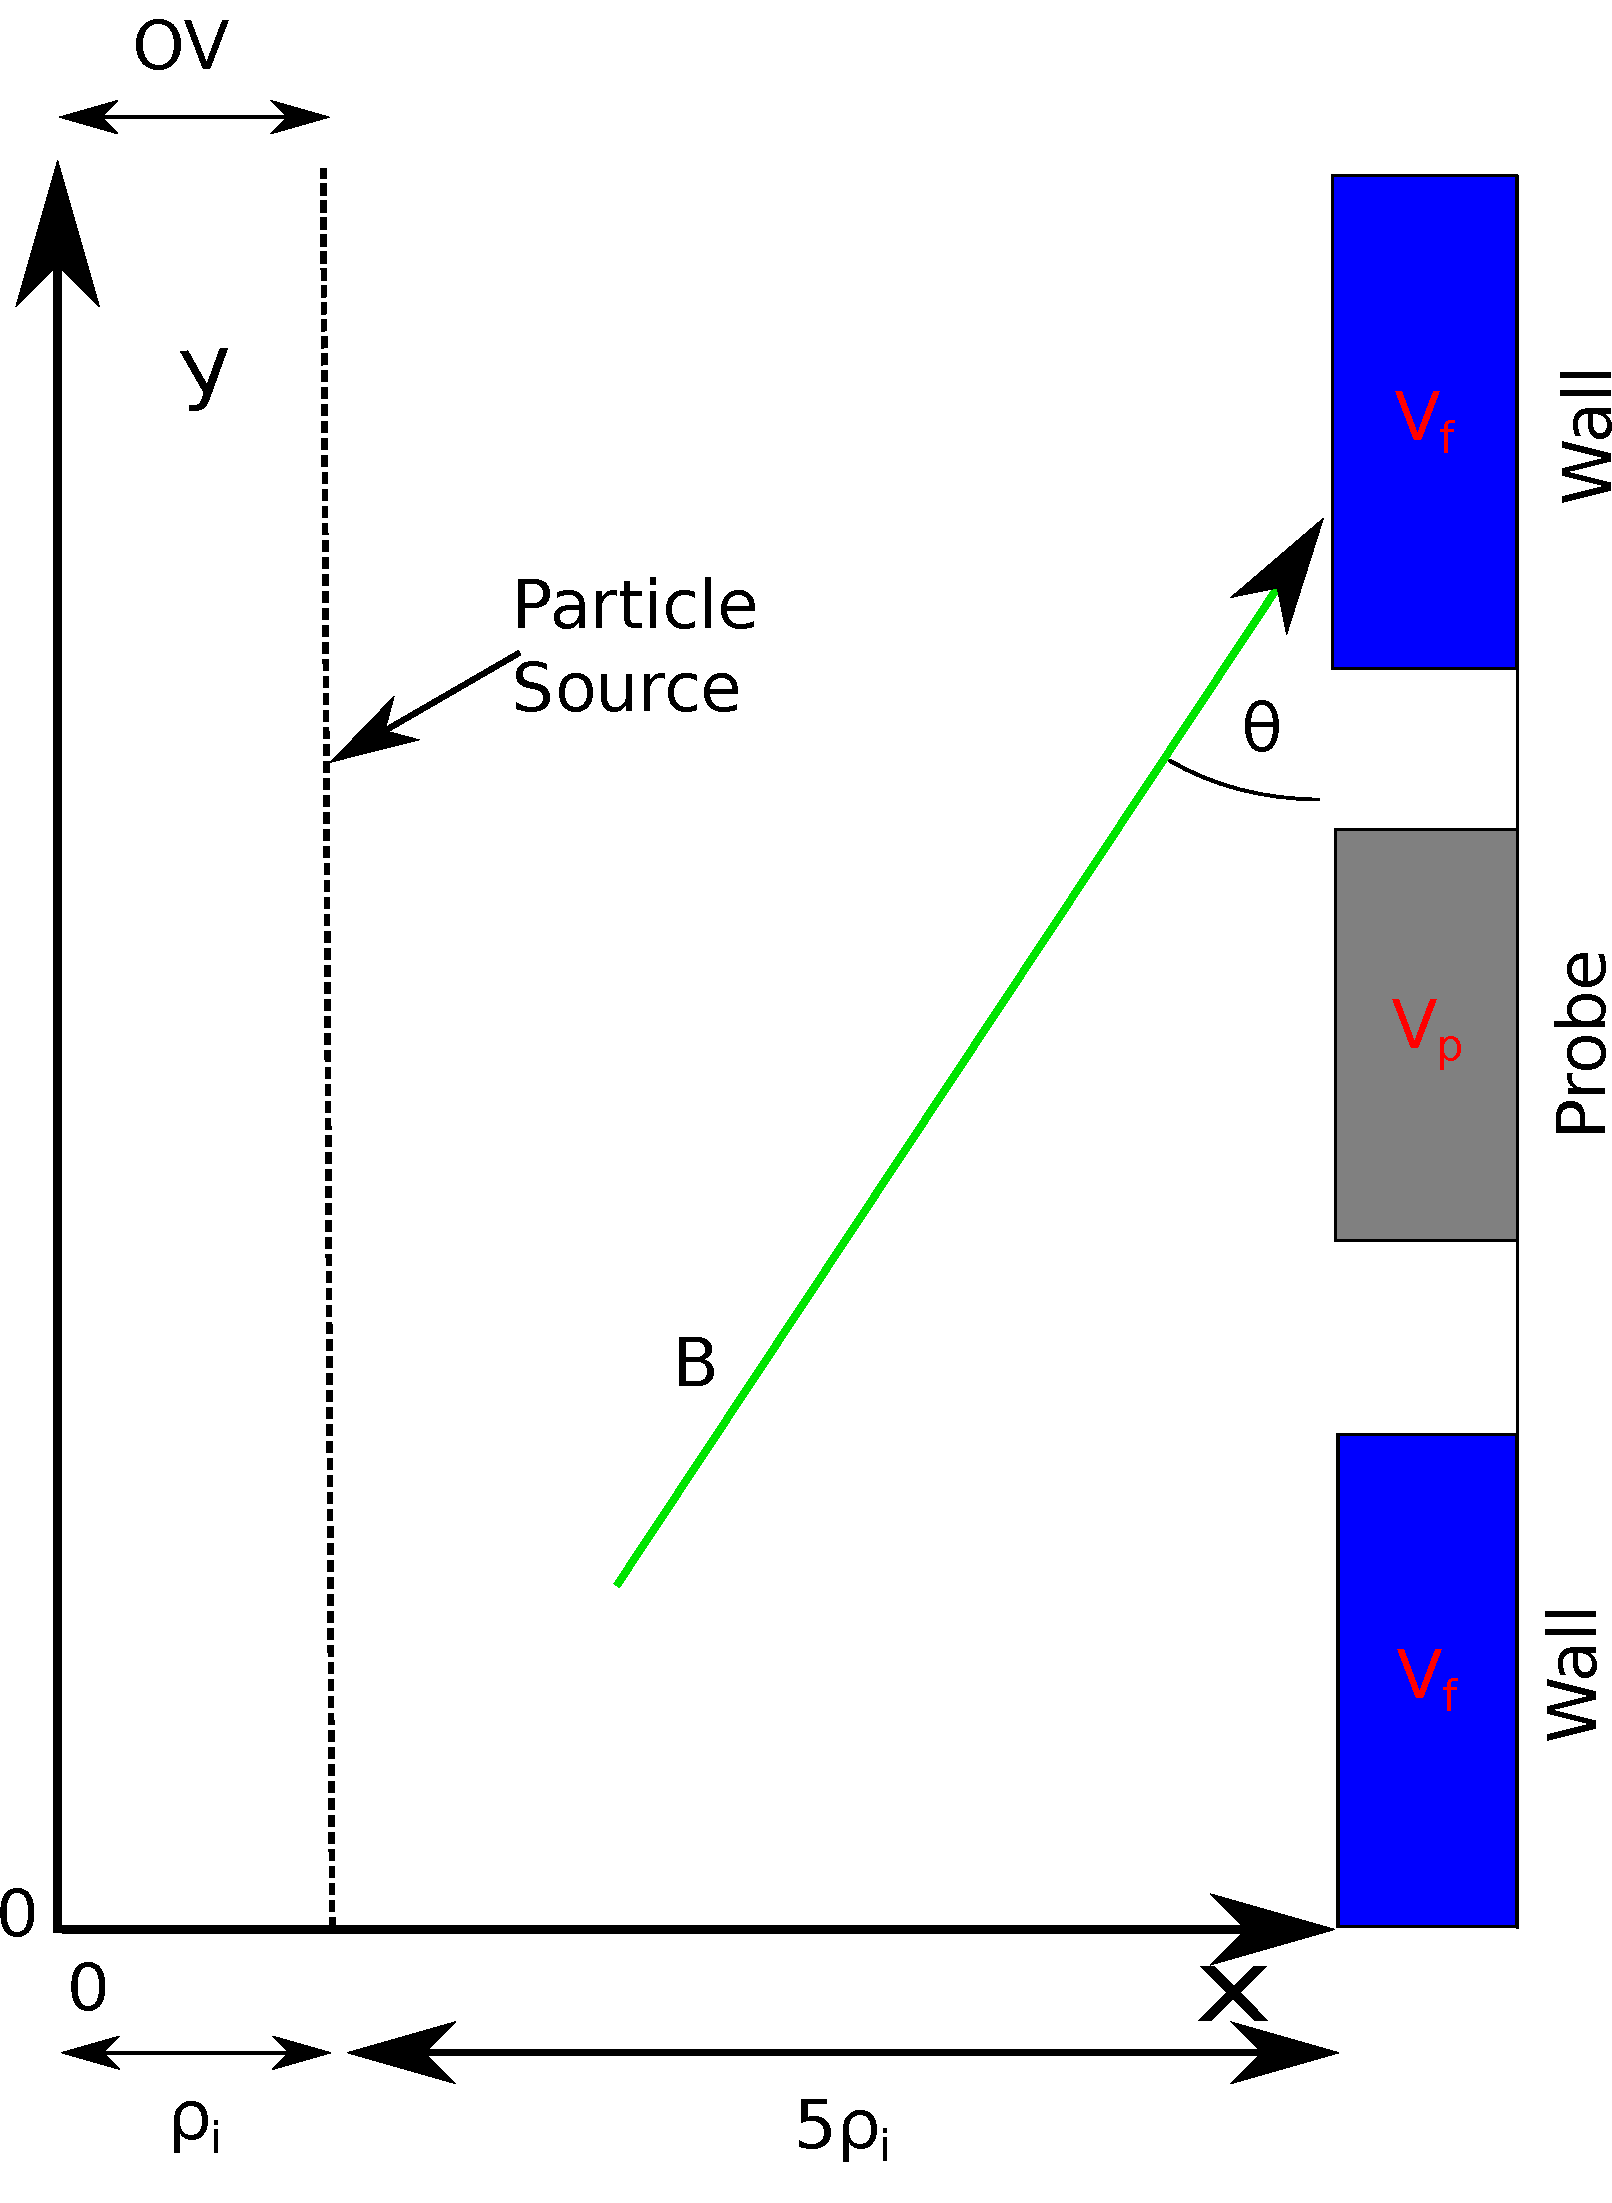
\includegraphics[width=8cm, height = 8cm]{gap_model.pdf}
	\caption{The simulation domain. Particles are injected in the source region to replenish those lost to the wall. The magnetic field makes an angle $\theta$ to the probe surface. An additional Larmor buffer region is included to ensure only particles with parallel velocity moving away from the probe are deleted.}
	\label{fig:2D_domain}
\end{figure}

\begin{table}[]
	\centering

	\begin{tabular}{c|c|c}  %{lllll}
		 &  &  \\ % \\ \hline 
		Magnetic field strength $B$             & 0.41 T                                               \\
		Magnetic field inclination $\theta$                & $12^{\circ} $      \\
		Plasma density $n_0$               & $6.4 \, \times \, 10^{18} \, m^{-3}$ \\ 
		Electron temperature $T_e$ &      $ 6$ eV     \\ 
		Ion temperature  $T_i$ &     $6$ eV  \\  
		Ion Larmor radius $\rho_i$  &  $0.42$ mm  \\
		Electron Mass $m_e$ &  $9.11 \times \, 10^{-31}$ kg \\
		Ion Mass $m_i$ &  $900 \hspace{1mm} m_e$ \\
		Ion Charge $Z$ & $1.6 \times \, 10^{-19}$ C \\
		Probe Length $L$ & $2.38$ mm \\
	\end{tabular} 
		\caption{Typical plasma parameters used in the simulations of FMPs on MAST. }
		\label{tab:sim_parameters}
\end{table}




Before exploring the effects of the gap on charged particle collection it was necessary to benchmark the model developed in VSim against the simulations carried out in \cite{Bergmann-2002}. Simulations without the probe-wall gaps were carried out with VSim. The results of these simulations are presented in the following section. 

\section{Validating the Model}
\label{Section:benchmark}
In the VSim simulations a floating potential on the wall develops over time as charge is deposited on the walls by the absorbed particles. This differs from the method deployed in \cite{Bergmann-2002}, in which multiple 1-D simulations were carried out to determine the potential at which net zero current reached the wall, this potential was then set as a prescribed boundary condition to the floating walls in the 2-D simulations. 
Presented in this section are results from VSim using the same simulation domain as that of \cite{Bergmann-2002}. These results aid in understanding the particle collection of FMPs and provide a means to benchmark the code. These results are compared to results obtained in both \cite{bergmann_1994} and \cite{Bergmann-2002}. The following results are obtained for a plasma of density  $n_0$ = $6.4 \, \times \, 10^{18} \, m^{-3}$, where $n_0$ refers to the density at the entrance to the MPS, a temperature of $T_e = T_i = 6$ eV, an inclination angle $\theta = 12^{\circ}$ and a probe bias voltage $V_{probe} = - 70$ V.

By plotting the density along lines perpendicular to the wall, the MPS and DS can be easily identified. The variation of density along two lines is shown in figure \ref{fig:Densities}, one in front of the probe and the other in front of the floating wall. The solid lines represent the particle densities in front of the probe and dashed lines represent the density in front of the wall. In order to obtain the density in front of the floating wall, the density was calculated on both sides of the probe and then averaged.

\label{Section:benchmark}
\begin{figure}[H]
	\centering
	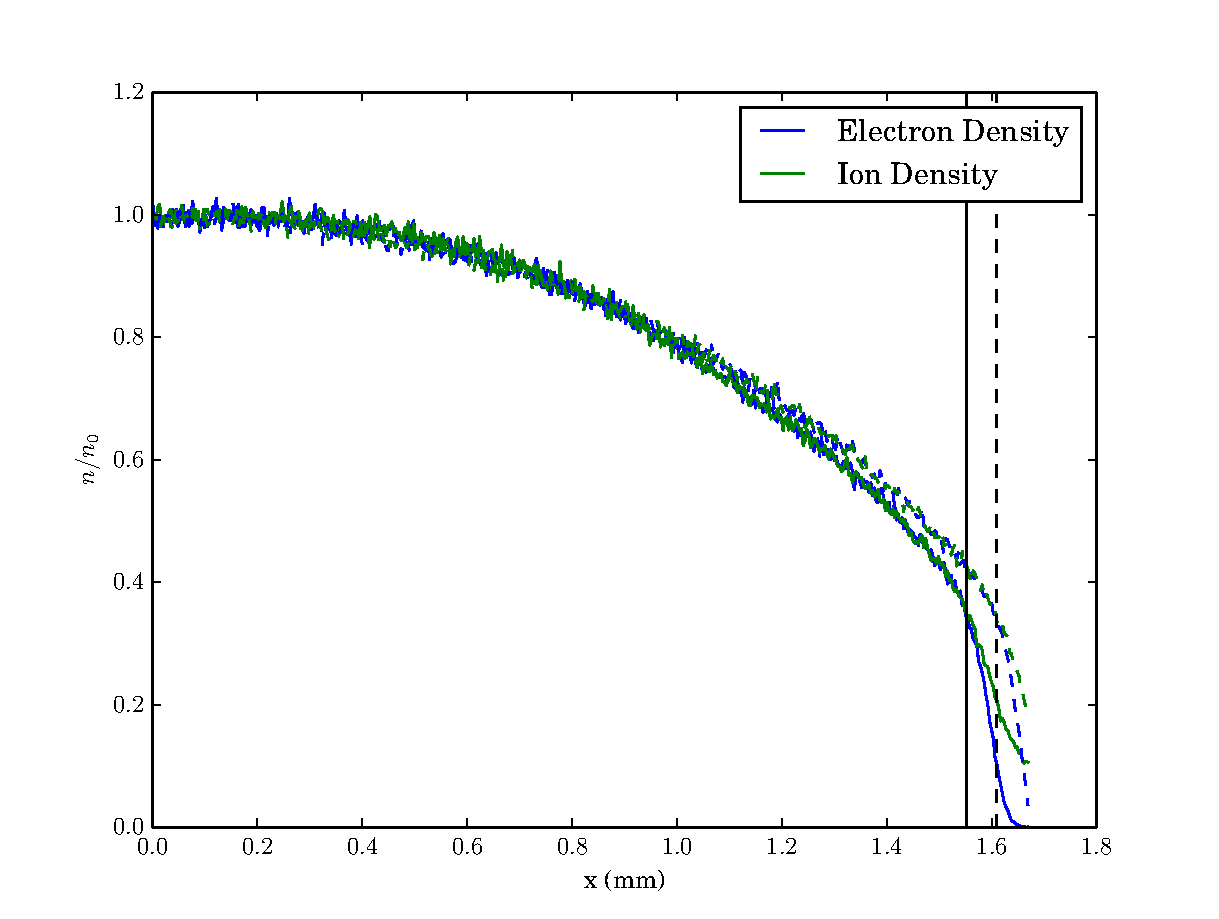
\includegraphics[width=0.9\textwidth, height = 8cm]{mps_densities.pdf}
	\caption{The ion density (green) and electron density (blue) along a line perpendicular to the wall. Densities are normalised with respect to the density at the entrance to the MPS. Solid lines represent the density in front of the centre of the probe, dashed lines represent the density in front of the floating walls. The vertical lines represent an approximate beginning of the DS, where quasi-neutrality breaks down. }
	\label{fig:Densities}
\end{figure}

The quasi-neutral MPS can be easily distinguished from the DS where the electron density tends to zero. The black, vertical lines represent an approximate location of the entrance to the DS where quasi-neutrality breaks down. The enhanced thickness of the probe's DS can be seen. The density drop across the MPS is observed for both lines, with the drop occurring earlier in front of the probe. This occurs earlier because the DS in front of the probe is thicker and so the probe's MPS begins further from the wall. The density at the entrance to both DS' is approximately the same. As has been discussed, this density drop is a key part of the fluid model \cite{fluid_model} and has been observed in PIC simulations \cite{bergmann_1994}, \cite{Chodura}. 

The effect of the enhanced sheath thickness on ion current can be observed in figure \ref{fig:fluxes}. A large peak is observed at the leading edge of the probe, as ions hit the side of the enhanced DS sheath and are focused on to the probe. The probe is biased sufficiently negatively such that no electrons reach the probe surface. The effects of the bifurcation point in the ion trajectories are observed with a large reduction in current reaching the trailing edge of the probe.



%Just to right of probe no electrons can their due to shadowing so ions are the more mobile species, wall charges very positively. Even if the wall potential is fixed, we see a bump in the electron flux is this a larmor effect? This bump is then matched in the ion current as it has to follow the elctron current. we see have an effect on the potential the wall reaches too. Electron bump caused due to their attraction to the huge positive potential - No because still happens in fixed vf model

 %Need to talk about equal fluxes at wall surfaces unlike bergmanns, trailing edge, fact the electrons are shielded from wall but ions can reach it, maybe get that y density plot in front of wall, see if we can see shadowing effect, plot of the potential CHECK DENSITY PLOT FOR THE VF FIXED CASE, DO WE SEE CLEAR SHADOW REGION. WHAT MAY HAPPEN IS THAT SHADOW REGION FORMS IN MY MODEL BUT THEN IONS HIT THE WALL MORE THEN ALECTRONS CAUSE IT TO CHARGE POSITIVELY AND PERTURB THE IONS, STOP THEM HITTING THE WALL ETC 
\begin{figure}[H]
	\centering
	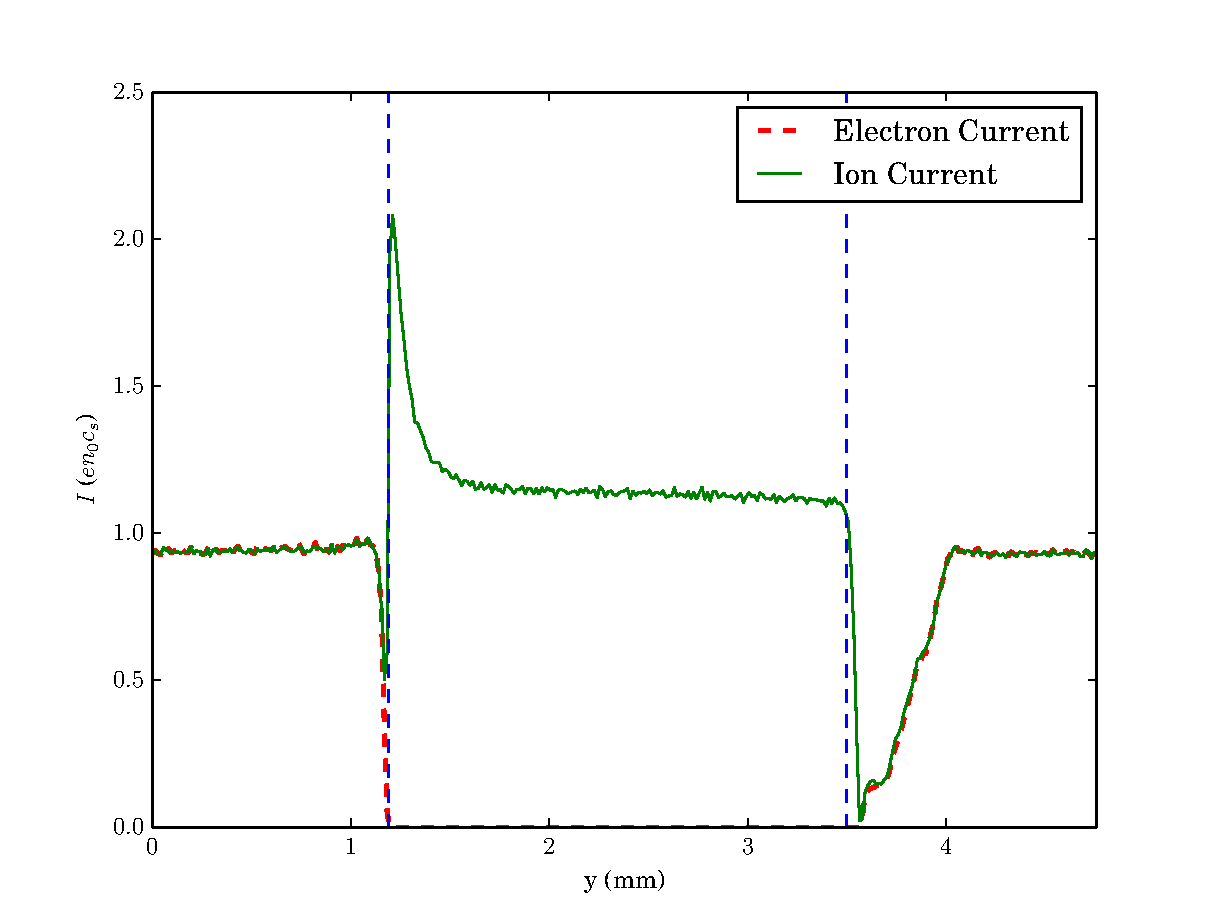
\includegraphics[width=0.9\textwidth, height = 8cm]{both_fluxes_150V.pdf}
	\caption{The ion current (green, solid) and electron current (red, dashed) reaching the wall. The currents are normalised by $I_0$. The edges of the probe are shown in dashed, vertical lines.  }
	\label{fig:fluxes}
\end{figure}
As observed in \cite{bergmann_1994}, there is a region behind the trailing edge of the probe, that is depleted of electrons. The electrons are unable to access this region as they are tied to magnetic field lines, electrons that would reach this region are reflected by the negative potential of the Debye sheath. This region can be distinguished when plotting the particle density in front of the wall as shown in figure \ref{fig:density_y}. As the walls are allowed to establish a floating potential, there are equal fluxes of ions and electrons at all points along the length of the wall apart from at the very edge of the right hand side of the probe, as ions are the only species capable of hitting this region of the wall. A positive potential therefore develops at this point to attract electrons and repel ions. The potential structure along the wall is shown in figure \ref{fig:potential}.

\begin{figure}[]
	\centering
	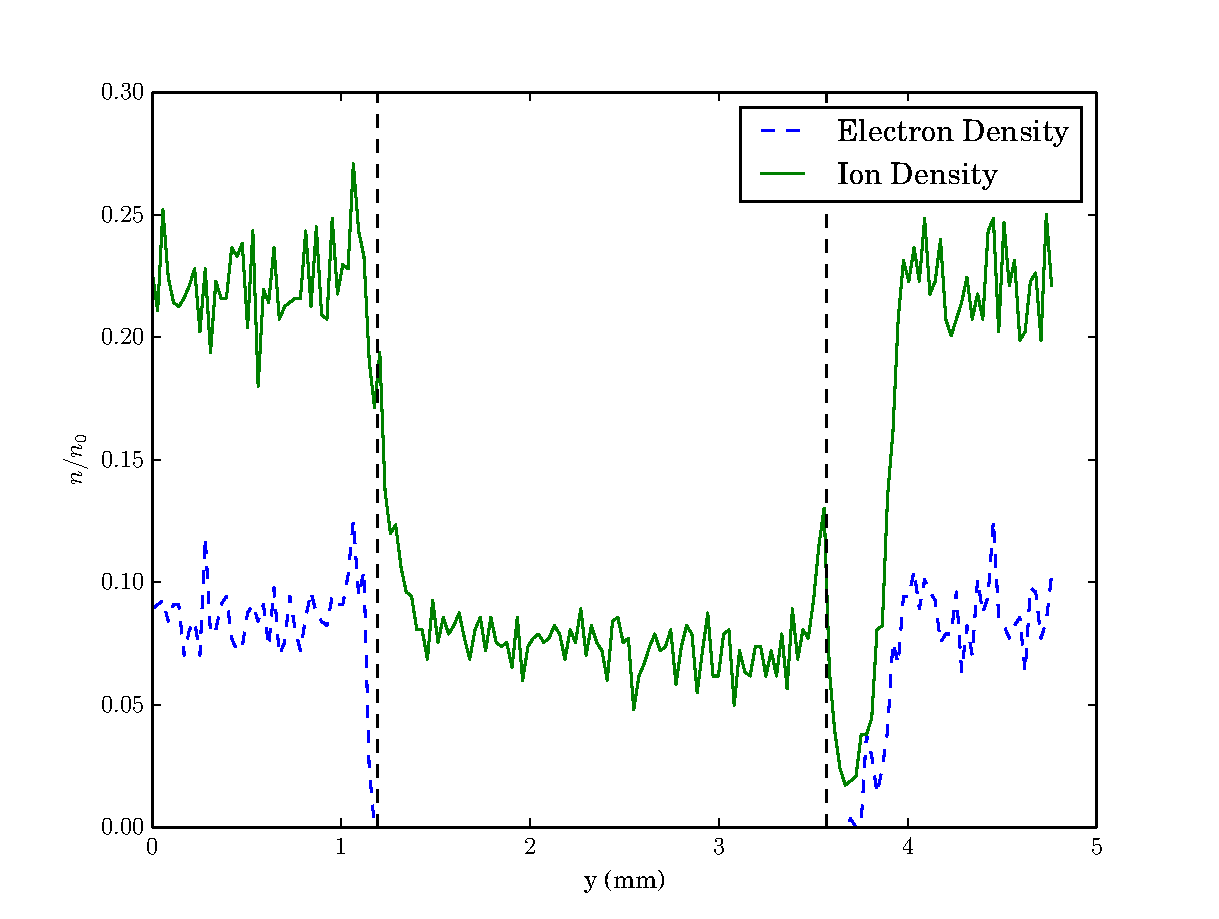
\includegraphics[width=0.9\textwidth, height = 8cm]{density_in_front_of_wall_150V.pdf}
	\caption{The ion density (green, solid) and electron density (blue, dashed) in front of the wall. The densities are normalised by the density at the entrance to the MPS. The edges of the probe are shown in dashed, vertical lines.  }
	\label{fig:density_y}
\end{figure}

\begin{figure}[]
	\centering
	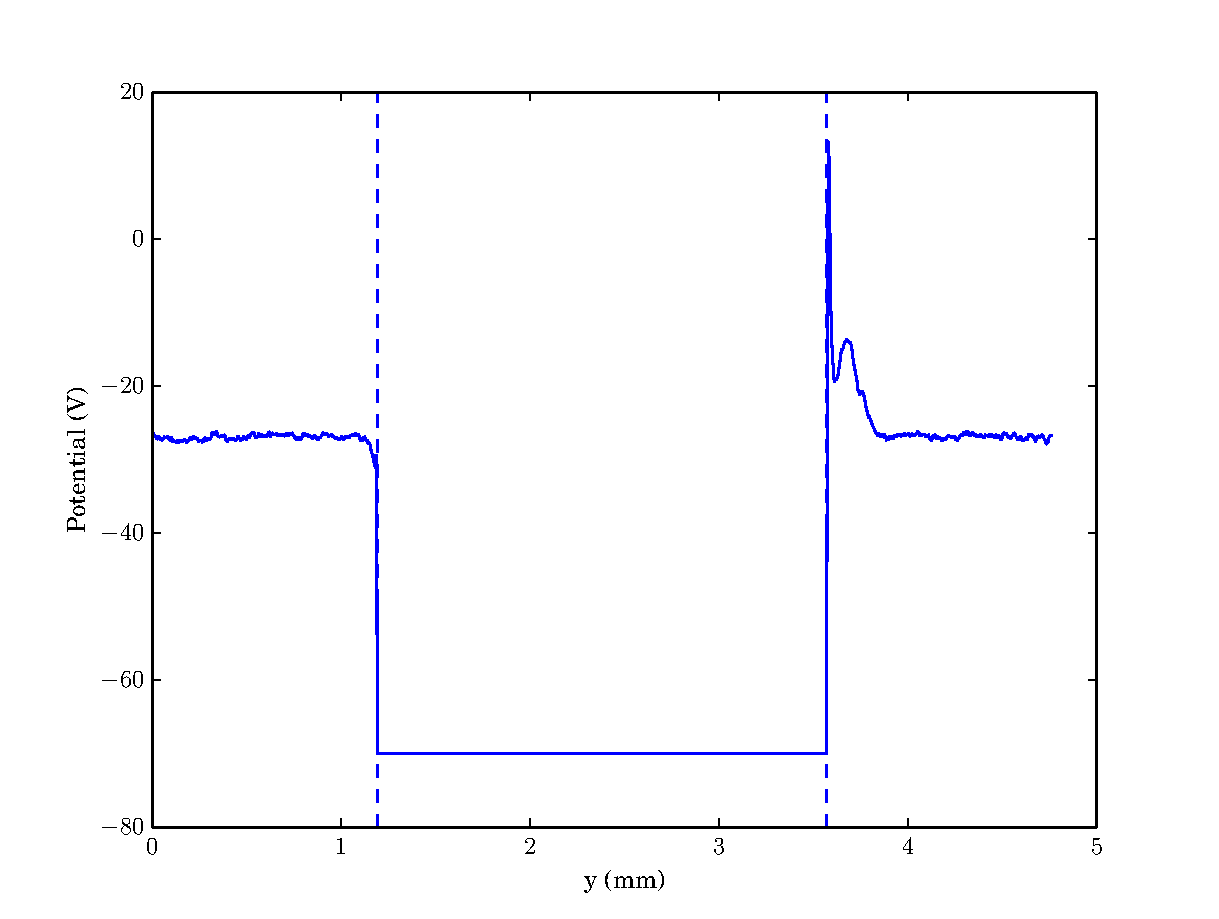
\includegraphics[width=0.9\textwidth, height = 8cm]{potential_on_wall.pdf}
	\caption{The potential profile along the wall. }
	\label{fig:potential}
\end{figure}

In order to measure the value of the coefficients $c_1$ and $c_2$ in equation \ref{eq:sheath_expansion} a value of $a$ is required for multiple field inclination angles, keeping the other plasma parameters constant. The value of $a$ can be extracted from the ion current collected by the probe at different bias voltages. From equation \ref{eq:IV}, taking the ion current component
\be 
I_{ion} = I_0 + I_0a{\left|V\right|}^{3/4}
\ee
Plotting the ion current against ${\left|V\right|}^{3/4}$ then gives a straight line, with the y-intercept equal to $I_0$ and the gradient equal to $I_0 a$ as shown in figure \ref{fig:a_no_gap}. 



\begin{figure}[H]
	\centering
	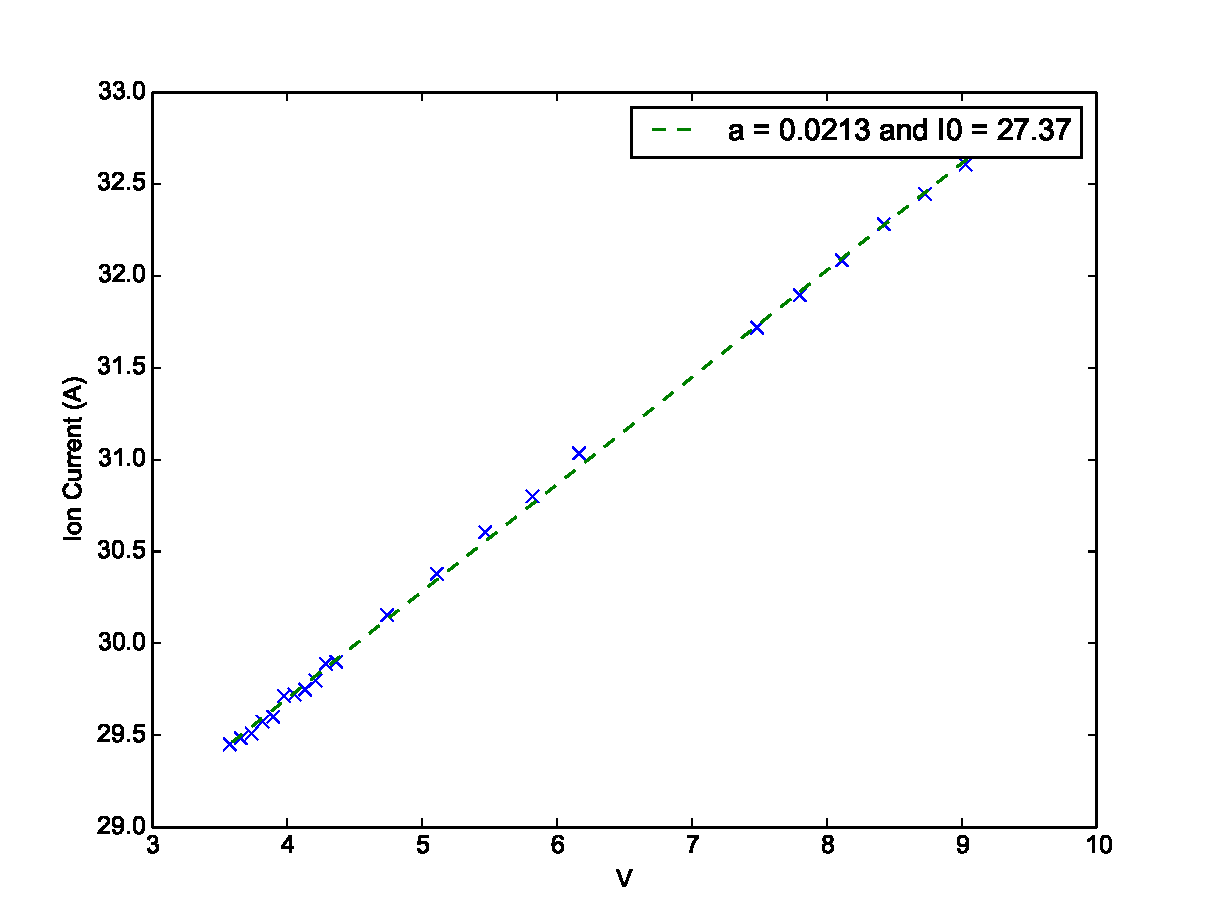
\includegraphics[width=0.9\textwidth]{a_no_gap.pdf}
	\caption{The ion current collected by the probe at different bias voltages. }
	\label{fig:a_no_gap}
\end{figure}

To validate the VSim PIC simulations, this procedure was carried out for three different angles of inclination. From equation \ref{eq:IV}, it can be seen that a plot of $a L {(\sin \theta)}^{1/2}$ against $\cot \theta$ results in a straight line graph with $c_1$ equal to the y-intercept and $c_2$ equal to the gradient. Figure \ref{fig:no_gap_c1} shows the VSim results agree well with those of \cite{Bergmann-2002}.

\begin{figure}[H]
	\centering
	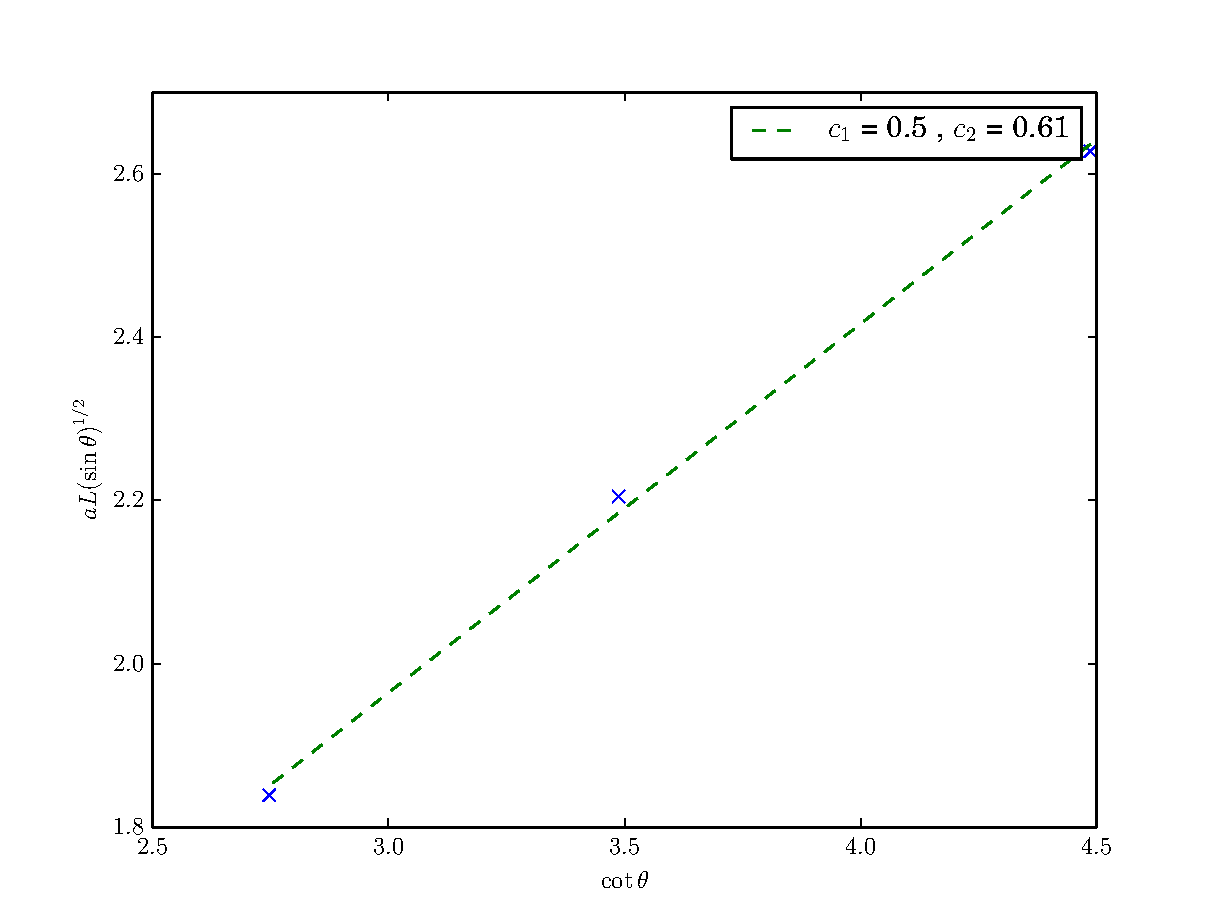
\includegraphics[width=0.9\textwidth, height = 8cm]{no_gap_c1_c2.pdf}
	\caption{The product of parameter $a$ extracted from the I-V characteristic multiplied by $\sqrt{\sin \theta}$ and the length of the probe (in units of $\lambda_D$ against $\cot \theta$. }
	\label{fig:no_gap_c1}
\end{figure}

In summary, the transition from the MPS to the DS can clearly be seen in the simulation results. As with \cite{bergmann_1994}: an enhanced sheath thickness in front of the probe, relative to the floating wall is observed; the thicker sheath leads to an ion focusing effect at the leading edge of the probe; whilst electrons, that are tied to magnetic field lines, cannot access a region behind the probe.
The floating condition used in VSim ensures equal fluxes of both species to the wall and results in a potential structure behind the trailing edge of the probe that is not observed in \cite{bergmann_1994}. This does not appear to affect the charged particle collection by the probe as good agreement with the model presented in \cite{Bergmann-2002} has been found.


\section{Incorporating the Gaps}
After successful comparison with \cite{Bergmann-2002}, simulations were carried out including a gap between the probe and the wall, using the simulation domain shown in figure \ref{fig:2D_domain}.  The effect of the presence of a probe-wall gap becomes evident when plotting the current reaching each part of the wall, as shown in figure \ref{fig:fluxes_gap}. Both the leading edge of the probe and the face of the wall behind the trailing edge of the probe, upon which magnetic field lines end, see a large ion current. In the case of the probe, the increase in the ion current is much larger than that caused by the ion focusing effect. The effective collection area of the probe is increased as magnetic field lines terminate on the side of the probe. This is also the case for the face of the wall behind the trailing edge of the probe. The increased ion current here is matched by a higher electron current. The peak in ion current at the wall is lower than at the probe for two reasons. Firstly, the floating wall doesn't experience an ion focusing effect and secondly, as with the no-gap simulations, the particle density is reduced in a region behind the trailing edge of the probe. The particle density in front of the wall for the gap model is shown in figure \ref{fig:density_y_gap}.
\begin{figure}[H]
	\centering
	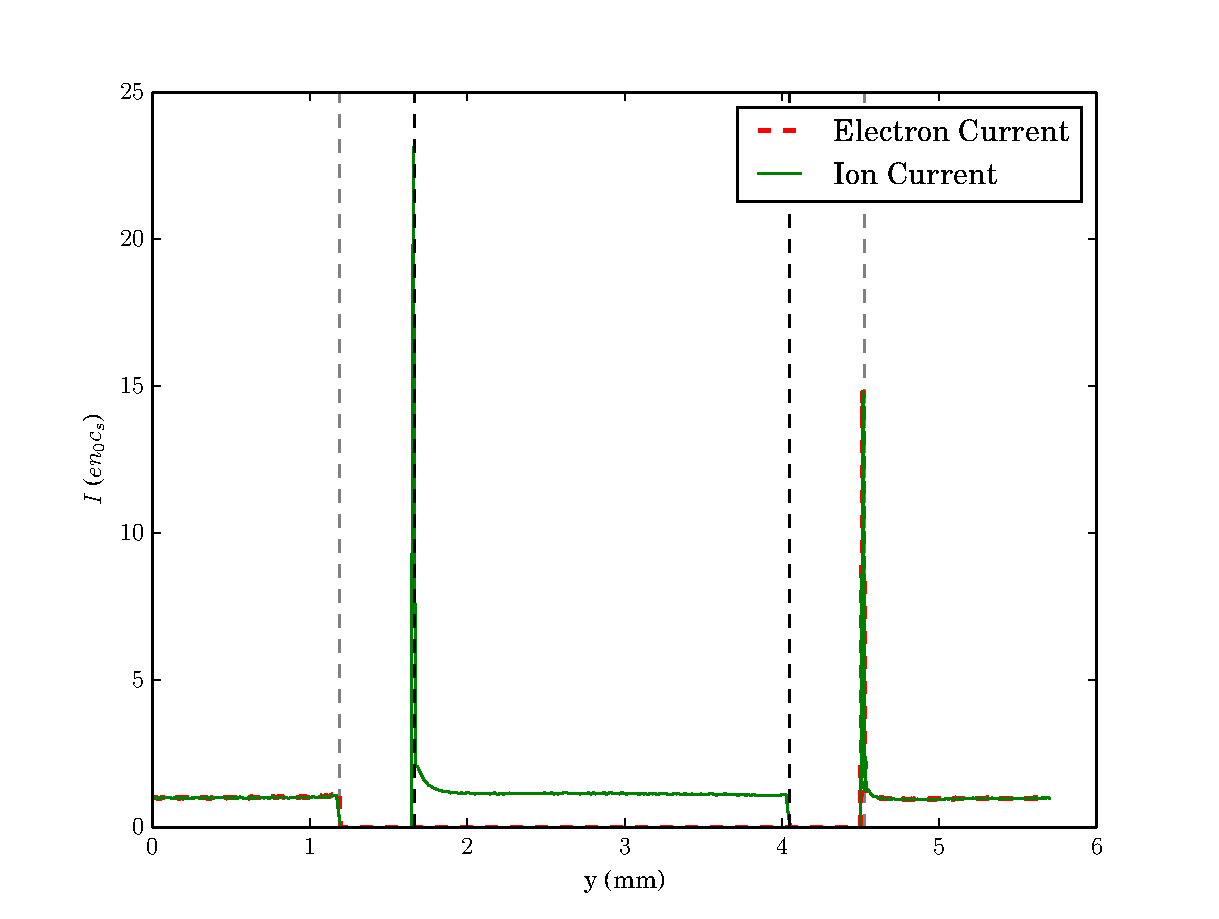
\includegraphics[width=0.9\textwidth, height = 7.5cm]{both_fluxes_gap.pdf}
	\caption{The ion current (green, solid) and electron current (red, dashed) reaching the wall. The currents are normalised by $I_0$. The edges of the probe (wall) are shown in black (grey),  dashed, vertical lines. }
	\label{fig:fluxes_gap}
\end{figure}

The densities in front of the wall and probe show the same trends as for the no-gap model. The ion density in front of the wall is higher than in front of the probe as this region is deeper into the probe's DS. The particle densities are much higher in front of the gaps where there is no surface for a build up of charge to develop and therefore no sheath forms. The lateral expansion of the probe's DS can be seen in a plot of the electrostatic potential in front of the wall as shown in figure \ref{fig:thicker_sheath}.

\begin{figure}[H]
	\centering
	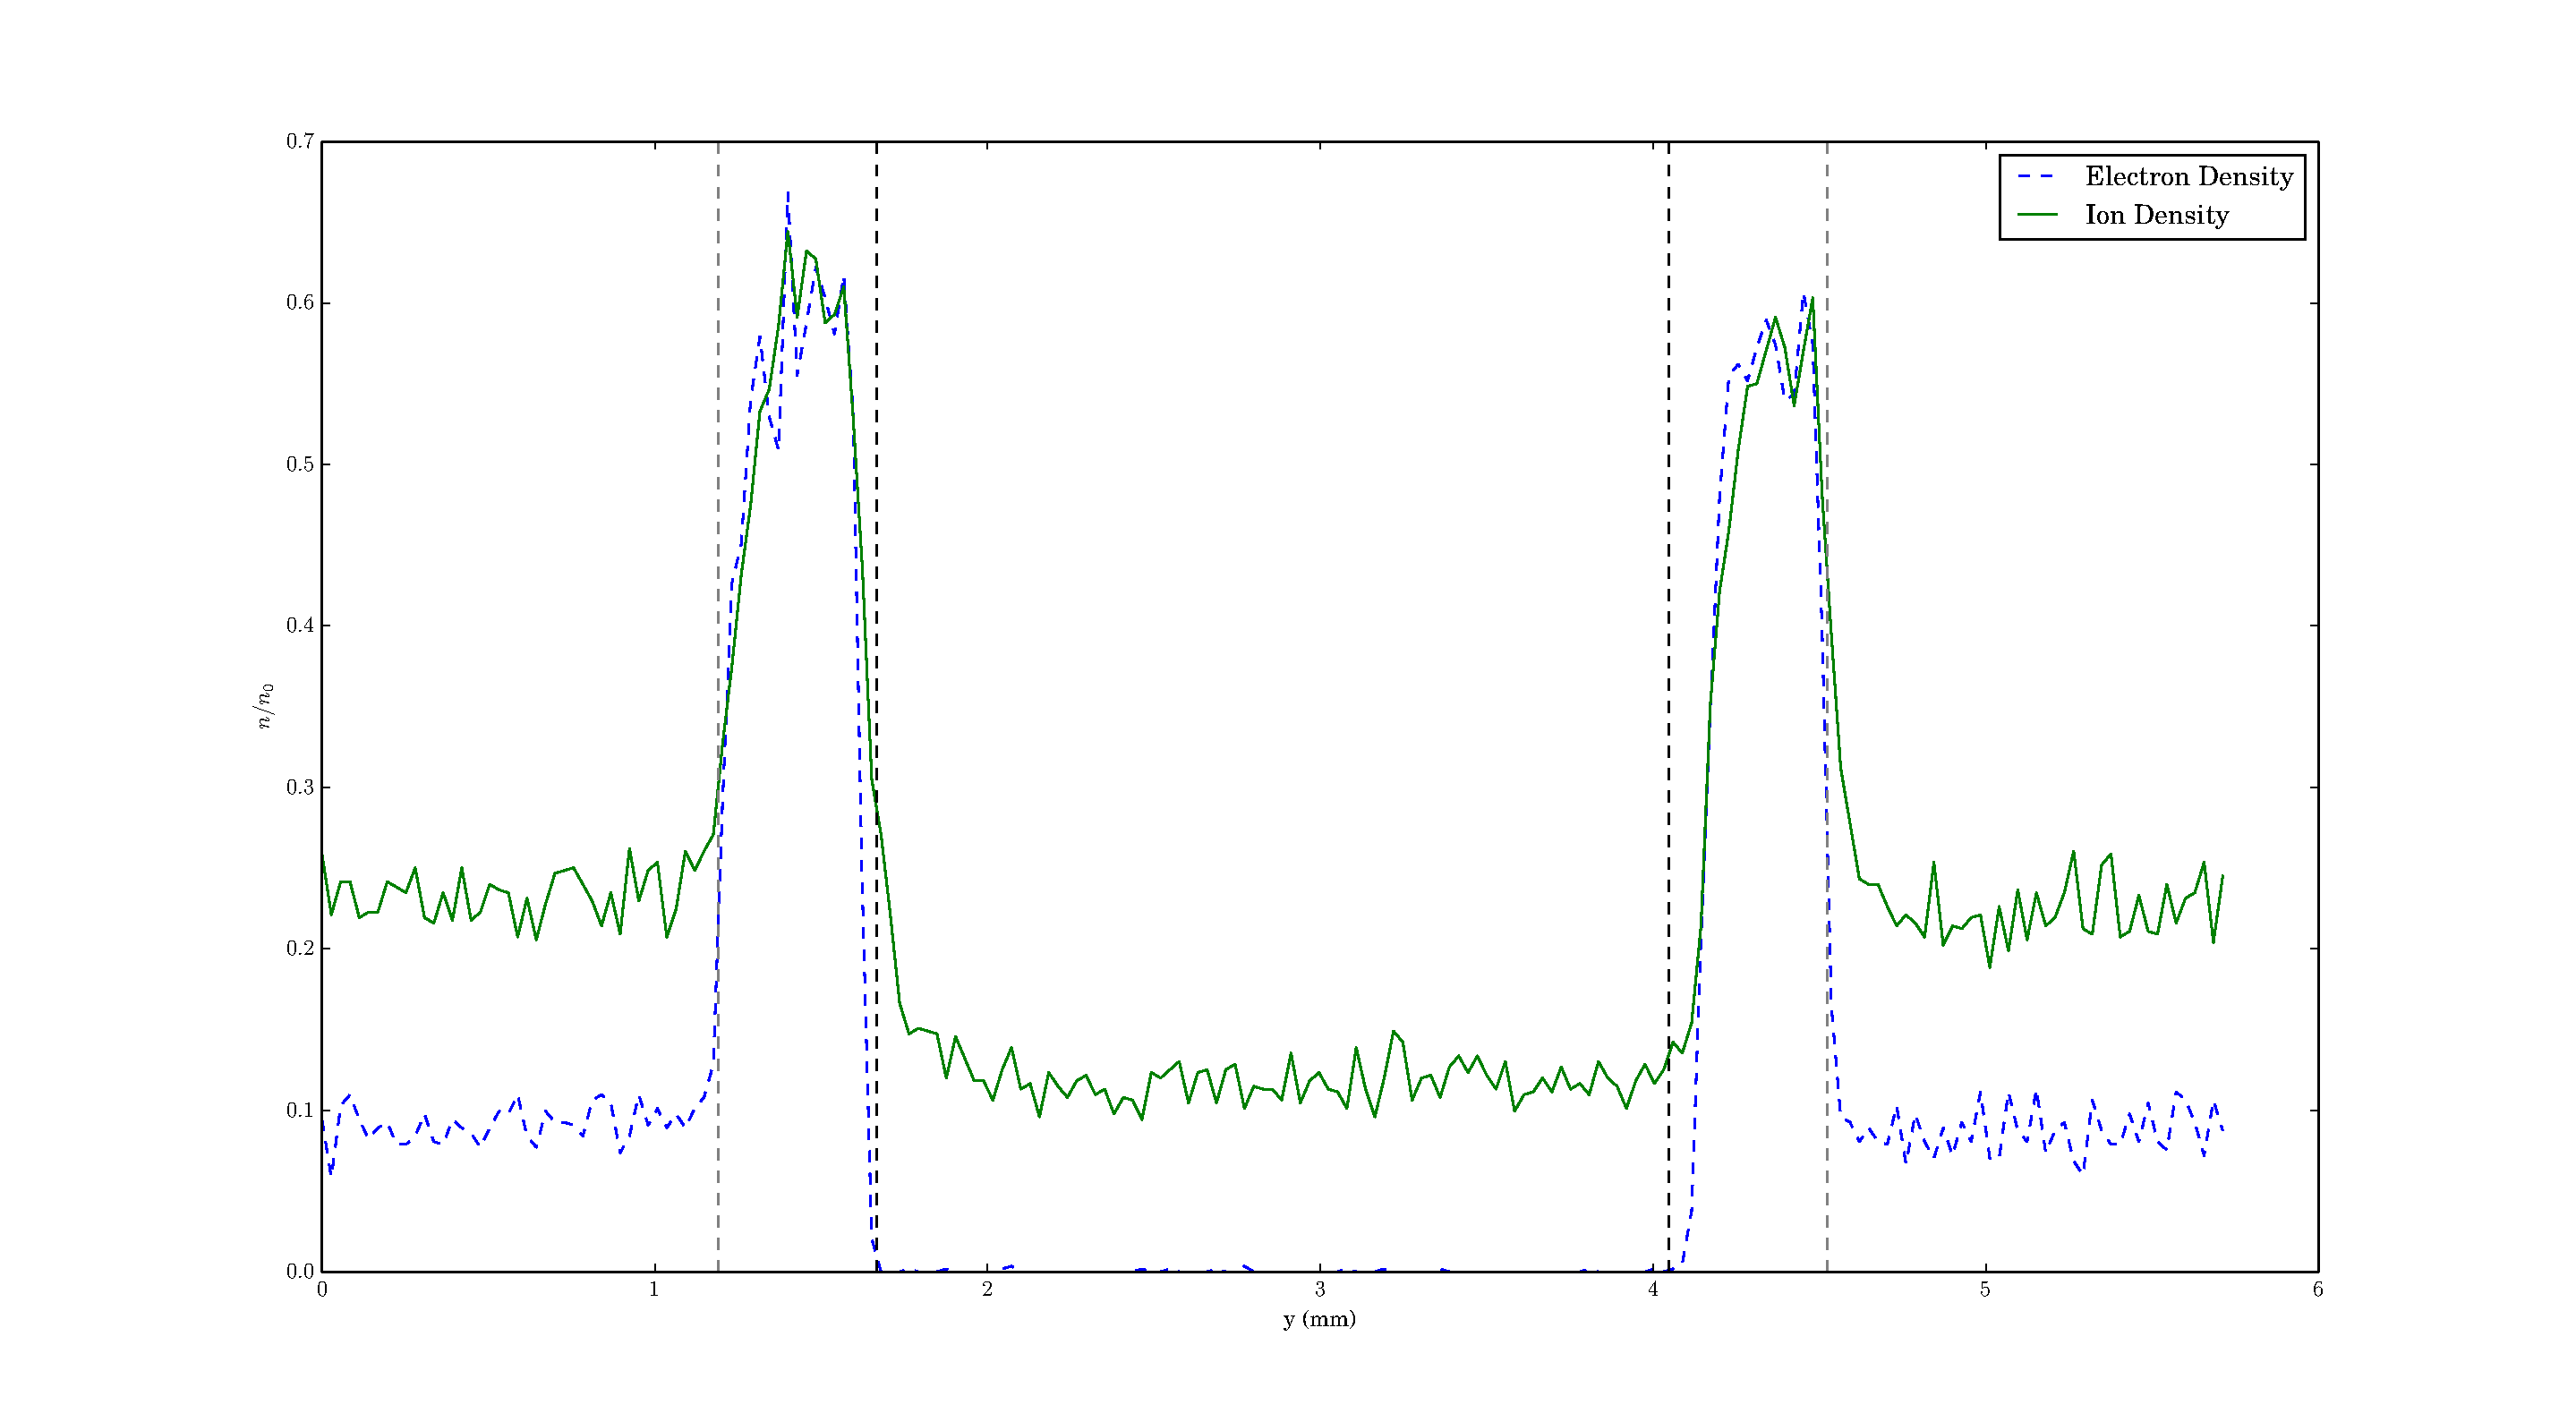
\includegraphics[width=\textwidth, height = 10cm]{density_in_front_of_wall_gap.pdf}
	\caption{The ion density (green, solid) and electron density (blue, dashed) in front of the wall. The densities are normalised by the density at the entrance to the MPS. The edges of the probe (wall) are shown in black (grey),  dashed, vertical lines.   }
	\label{fig:density_y_gap}
\end{figure}


\begin{figure}[H]
	\centering
	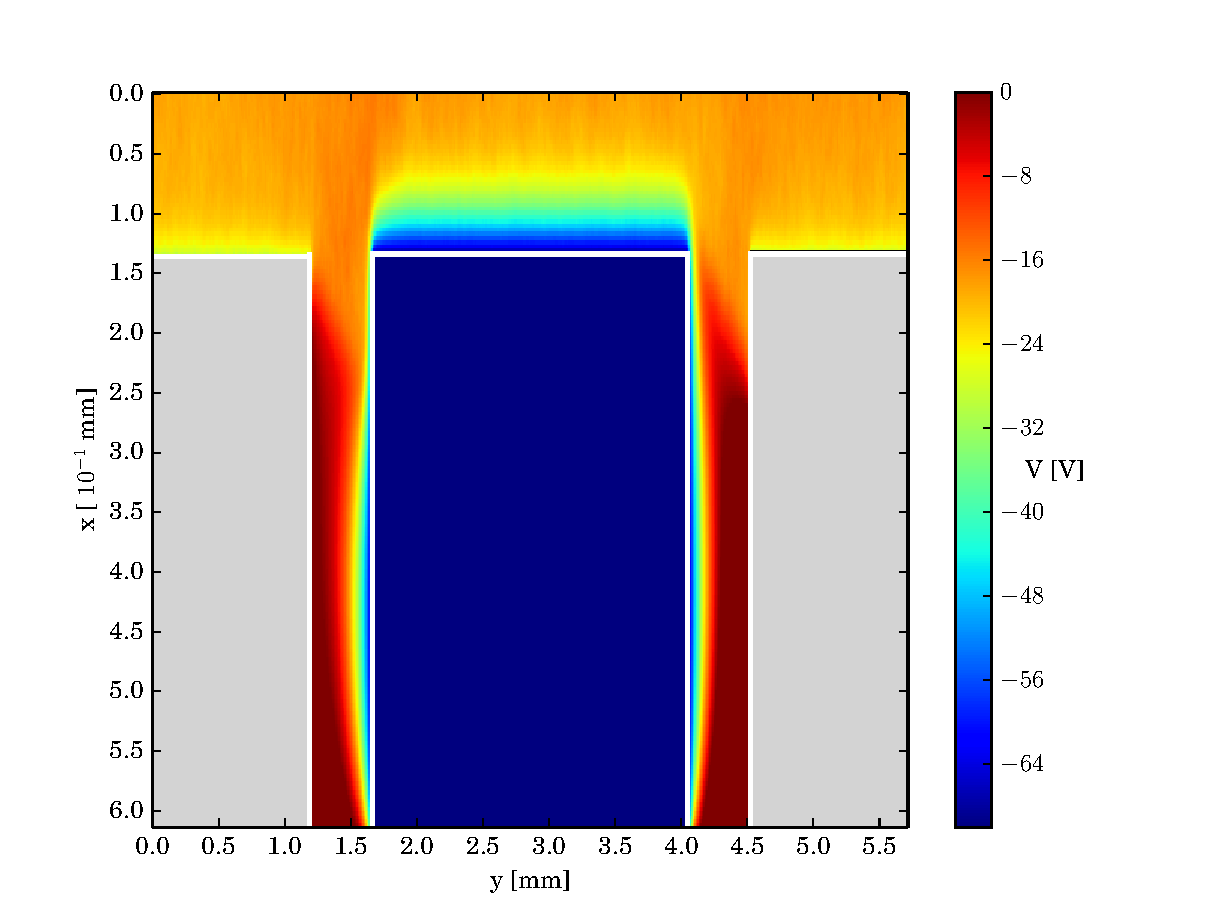
\includegraphics[width=0.9\textwidth]{potential_75V.pdf}
	\caption{The potential structure in front of the wall in a VSim simulation incorporating the gaps. The probe is biased negatively with respect to the surrounding floating walls (shown in grey), therefore the probe's DS is thicker than that of the walls. The thickness of the sheath is exaggerated in this figure due to the difference in scaling of the x and y-axes.}
	\label{fig:thicker_sheath}
\end{figure}

%\begin{figure}[H]
%	\centering
%	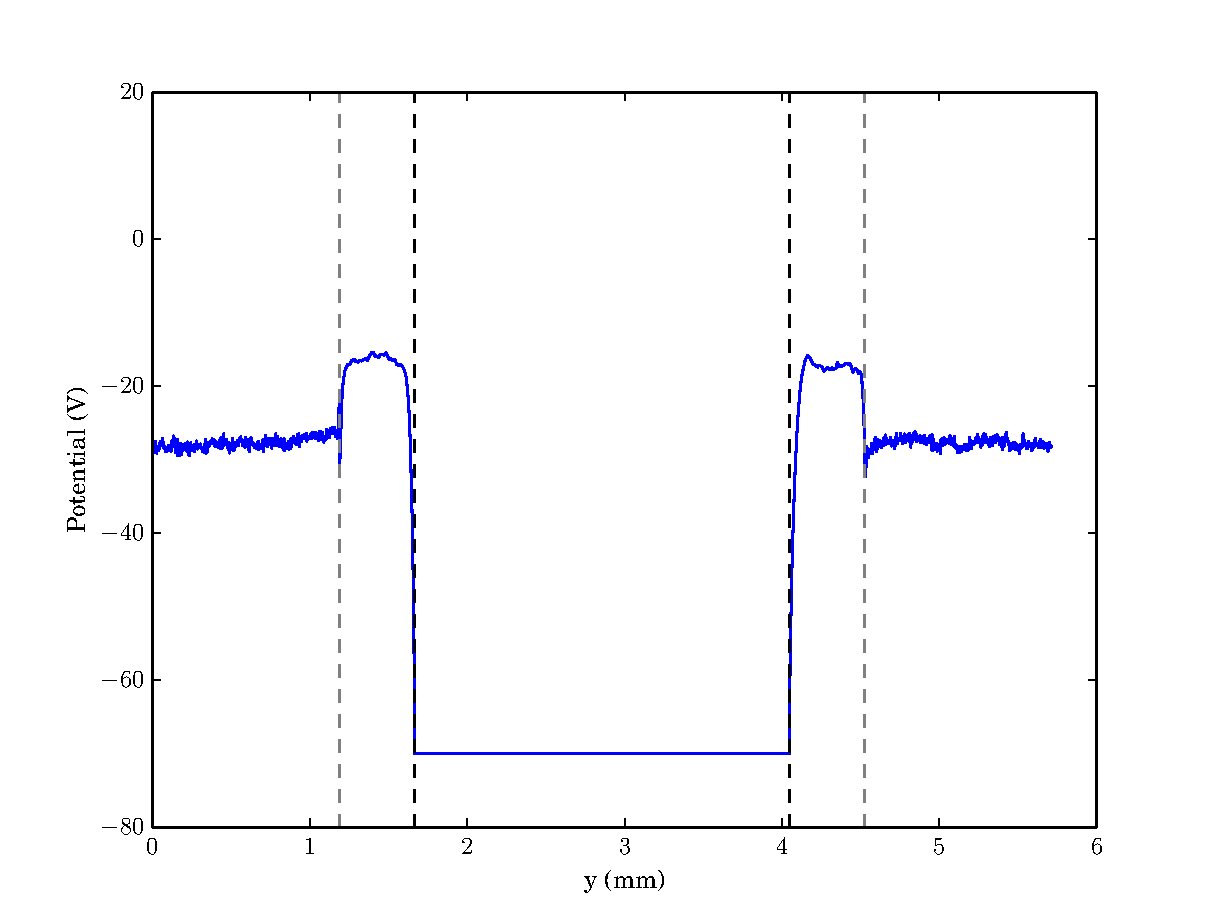
\includegraphics[width=0.9\textwidth, height = 8cm]{potential_on_wall_gap.pdf}
%	\caption{The potential profile along the wall. The edges of the probe (wall) are shown in black (grey),  dashed, vertical lines.   }
%	\label{fig:potential_gap}
%\end{figure}



The presence of the gap, exposes the side of the probe directly to plasma travelling along impinging field lines, increasing the effective collection length of the probe. The extent of this effect must be calculated in order to extract the correct plasma density from FMP data on MAST.



\section{Ion Collection and Estimation of the Electron Density}
The model of \cite{Bergmann-2002}, extended to include a gap between the probe and the divertor surface is shown in figure \ref{fig:sheath_model}. In front of the wall is a DS of thickness $\Delta_0$. The probe is biased more negatively than the floating wall and so has a DS thickness $\Delta$. The sheath expands laterally either side of the probe by the length $\delta$.
\begin{figure}[]
	\centering
	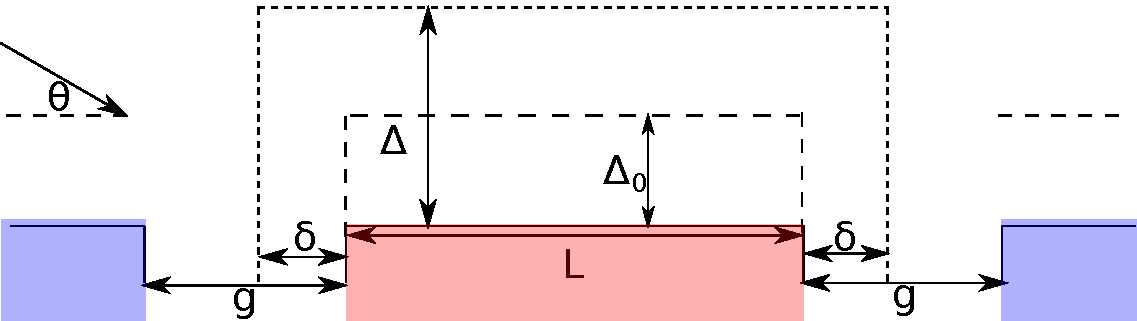
\includegraphics[width=0.9\textwidth]{sheath_model1.pdf}
	\caption{A model of the sheath in front of the FMP. The sheath is modelled as a rectangle. The floating wall has a sheath of thickness $\Delta_0$. For $V_{probe}$ $<$ $V_f$ the probe has an enhanced sheath thickness of $\Delta$ and a lateral expansion of $\delta$. }
	\label{fig:sheath_model}
\end{figure}
Two simulations were carried out with identical plasma parameters and probe bias voltages, one simulation with the gap and one without. Figure \ref{fig:increased_I0)} shows the effect of the gap on the collected ion current. The top line represents the current collected by the probe in the gap-model. From equation \ref{eq:IV} it can be seen that $I_0$ is the magnitude of the ion current at the point $V = 0$, when the probe is at floating potential. When $V= 0$, the DS thickness is the same in front of the probe as it is at the wall, the ion focusing effect therefore does not occur and the probe collects current over its projected length. The gap in between the probe and the wall exposes the left hand side of the probe to the plasma as presented in figure \ref{fig:sheath_model}. Magnetic field lines terminate on the side of the probe, therefore, the probe now subtends a larger flux tube. The length of the exposed side of the probe is given by $g \tan \theta$. Taking the projection of this length along the field results in $g \sin \theta$. As a result, the value of $I_0$ is increased by the factor $(L+g)/L$ from the no-gap case which would lead to an increase in the derived plasma density if not accounted for.
\begin{equation}
I_0 = q n c_s(L+g)\sin{\theta}
\end{equation}

\begin{figure}[H]
	\centering
	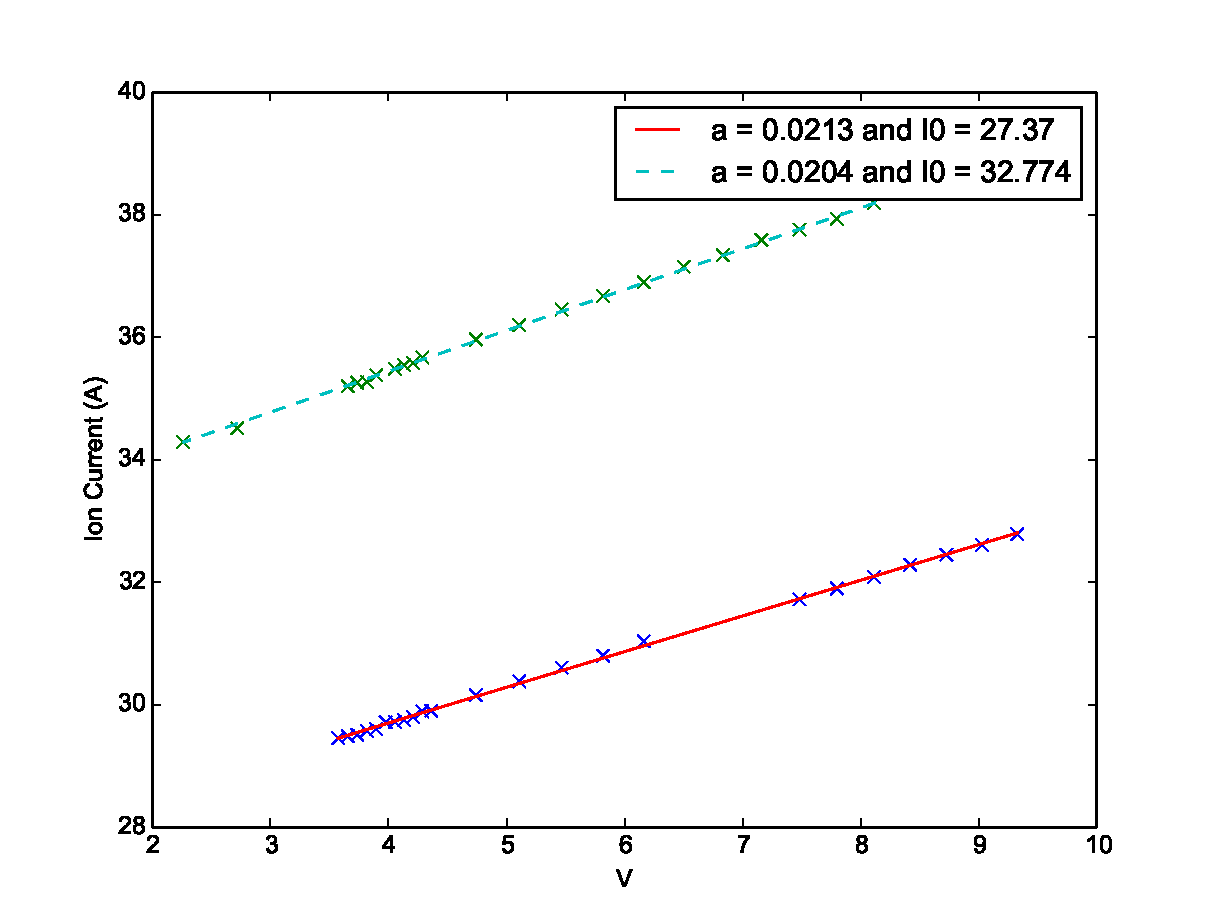
\includegraphics[width=0.9\textwidth]{ion_current_gap_no_gap.pdf}
	\caption{A plot of the ion current as a function of voltage applied to the probe. Top, dashed line represents the ion current in the gap model. Bottom, solid line is the current in the no-gap model.}
	\label{fig:increased_I0)}
\end{figure}
For MAST FMPs, $L=5$ mm and $g = 1$ mm. The presence of the gap therefore increases the collected ion current by $20\%$ for the MAST probes. As can be seen in figure \ref{fig:increased_I0)} the sheath expansion parameter is found to be lower for the probe in the gap-model. Following the derivation of \cite{bergmann_1994} for the sheath expansion parameter we have a new effective probe size  
 \begin{equation}
 \begin{aligned}
 L_{eff} ={} & [L +2\delta] \sin{\theta}  + (\Delta - \Delta_0) \cos{\theta}  + g\tan{\theta} \cos{\theta}  \\
 & = [L +2\delta + g] \sin{\theta}  + (\Delta - \Delta_0) \cos{\theta} 
 \end{aligned}
 \end{equation}
 %
 %, therefore smaller $a$, if c1 and c2 are at max values and you know theta and d then you would have to deduce debye length is smaller therefore density is higher.
 
 
The normalised current to the probe is then 
\begin{equation}
I_i/I_0 = \frac{L_{eff}}{(L+g)\sin{\theta}} = 1 +  \frac{2 \delta}{L+g} + \frac{(\Delta-\Delta_0)\cot{\theta}}{L+g}
\label{eq:normalised}
\end{equation}
From equations \ref{eq:IV} and \ref{eq:normalised} we have a new expression for the sheath expansion parameter 
\begin{equation}
a = \frac{2\delta + (\Delta-\Delta_0)\cot{\theta}}{(L+g)}V^{-3/4}
\label{eq:a_old}
\end{equation}
The size of the sheath surrounding the probe is proportional to the applied voltage and the local Debye length in front of the probe. This is larger than the Debye length far away from the probe due to the density drop in the MPS. Hence
\begin{equation}
\delta,\Delta \propto \frac{V^{3/4}}{\sqrt{\sin{\theta}}}
\end{equation}
Substituting these expressions into equation \ref{eq:a_old} gives 
\begin{equation}
a = \frac{c_1+c_2 \cot{\theta}}{\sqrt{\sin{\theta}}}\frac{\lambda_D}{L+g}
\label{eq:new_a}
\end{equation}
We expect to see a reduced sheath expansion parameter due to the presence of the gap, however, the predicted reduction from equation \ref{eq:new_a} is more severe than the measured reduction. Figure \ref{fig:alpha} shows the dependence of the sheath expansion parameter on $\theta$. Various probe lengths were simulated, for a range of $\theta$ typical to conditions on MAST. Each data point requires an I-V curve to be simulated in order to obtain a value for the sheath expansion parameter. Measuring $a$ for a range of probe lengths and field angles allows a measurement of $c_1$ and $c_2$ to be made. $c_2$ is the gradient of the line. As with \cite{Bergmann-2002}, we find $c_2$ depends on the ratio of the probe length to the Debye length, tending to 0.6 for larger probes. The y-intercept represents $c_1$, we find $c_1 \approx 0.9$ which is an increase over the previously reported value of 0.5. The inclusion of the probe-wall gap allows the probe sheath to expand laterally into a region of lower density than the bulk plasma. As a result of an increase in $c_1$, the reduction in the sheath expansion parameter for the gap model is not as severe as predicted. Taking into account the larger value for $c_1$ we find the sheath expansion parameter for probes in the gap-model is well described by equation \ref{eq:new_a}.

%The presence of the gap, exposes the side of the probe directly to plasma travelling along impinging field lines, increasing the effective collection length of the probe. If not taken into account, this effect will lead to an overestimation of the plasma density. The extent of this overestimation scales with gap width.  The effect of the reduced sheath expansion parameter will be discussed in section \ref{Sec:Experimental}. % Ideally the gap will be made as small as possible, machining limits?

%The model predicts $a$ values that are different to that of Bergmann's model but due to noise, cannot be resolved from experimental data. 

%COULD WE USE SOME SIMULATED DATA, FIT MY MODEL AND BERGMANNS MODEL, see what DENSITIES they predict. BERGMANN OVERSTIMATES DENSITY BY 20% 

  
%As well as providing a benchmark for comparison with Bergmann's simulations, the no-gap model allows   
%Not taking into account the gap Adds an error in  the density equivalent to the new length (L+g)/L  so gets worse for larger gaps, independent of angle
  
          \begin{figure}[H]
	\centering
	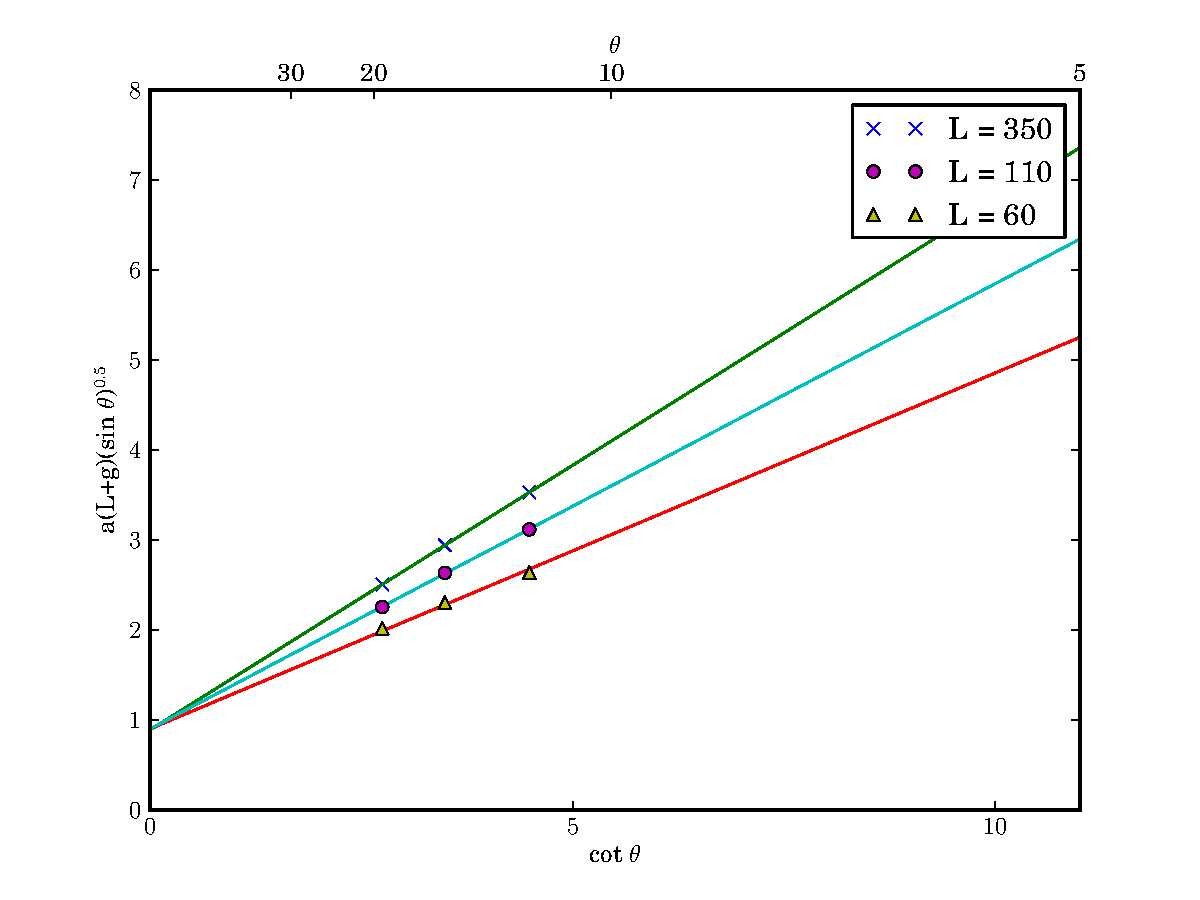
\includegraphics[width=0.9\textwidth]{c1_c2_plot.pdf}
	\caption{The product of the sheath expansion parameter $a$ obtained from the I-V characteristic multiplied by the probe length $L$ and the gap length $g$ (both in units of $\lambda_D$) and $\sqrt{\sin \theta}$ as a function of $\cot \theta$.}
	\label{fig:alpha}
\end{figure}

\section{Electron Collection and Electron Temperature Estimation}
In hot magnetised plasmas it is often assumed that the relation $I_e = I_0 e^{-V}$ holds provided the electrons have a Maxwellian velocity distribution. A restricted region of the IV curve, below the floating potential, is used to avoid problems of spuriously high $T_e$ measurements \cite{below_floating}, \cite{electrical_probes}, \cite{iv_safe_region}, \cite{pin-plate-pitts}. Once the ion current has been deducted from the total current it is then trivial to determine the electron temperature by plotting $\log{I_e}$ against $V_{probe}$ and measuring the gradient. 
Following the experimental procedure for the electron current to the probe in our simulations, it was observed that the probe measured $T_e$ values that were higher than the specified source temperature. This occurred in both simulations with and without the probe-wall gap provided $\theta \neq 90^{\circ}$. In simulations the electron current and ion current are known individually, therefore problems with non-saturation of the ion current will not influence the electron current measured in our simulations. The following results are presented for the simulations with the no-gap model, these were used to investigate the effect as the simulation domain consists of less grid cells and so the simulations are faster to run.
Examining the velocity distribution for electrons that are absorbed by the probe, reveals a significant portion of the electron current to the probe is made up of electrons that have a negative parallel velocity. This is shown in figure \ref{fig:absorbed_distribution}. These are electrons that have been reflected in the sheath and begin to move away from the probe, yet still reach the surface. 
\begin{figure}[]
	\centering
	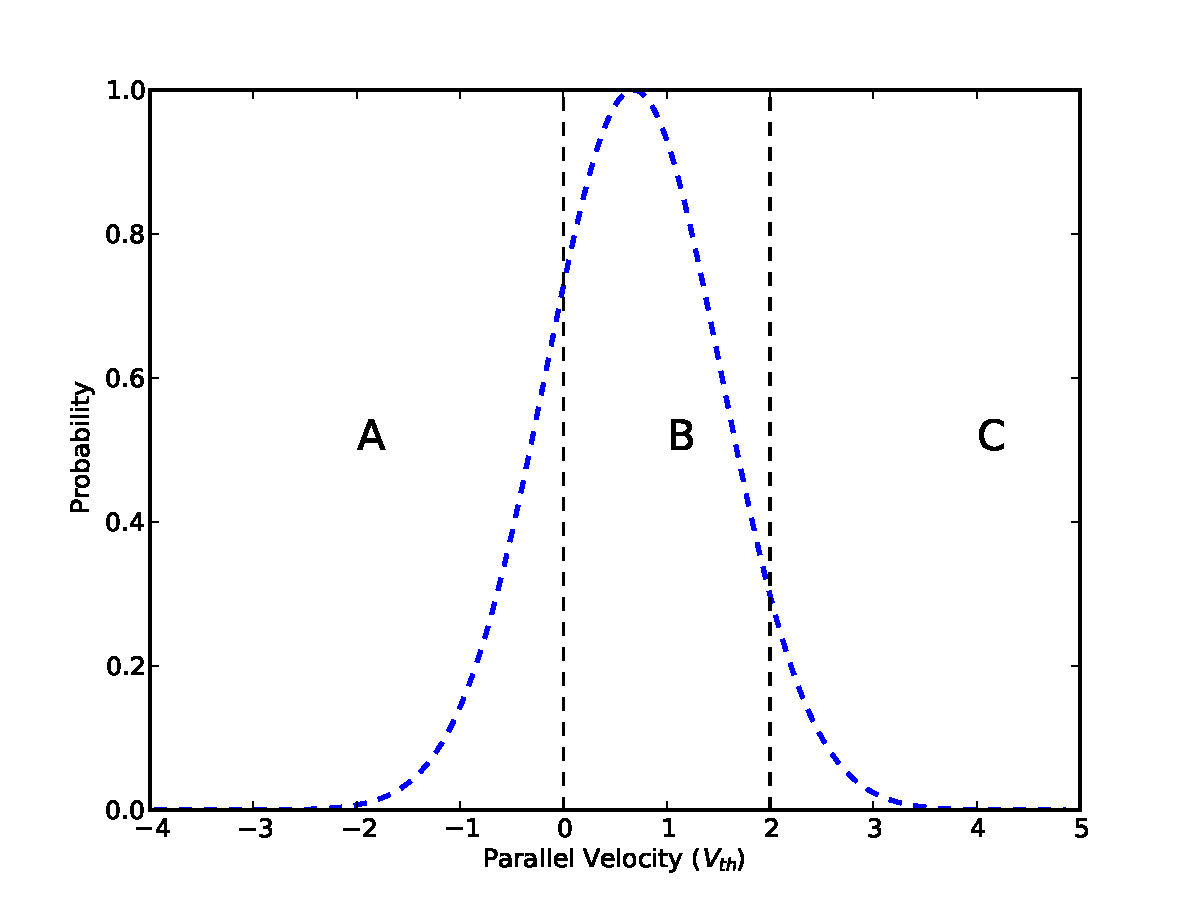
\includegraphics[width=0.9\textwidth , height = 8cm]{absorbed_distribution.pdf}
	\caption{The parallel velocity distribution of electrons that are absorbed by a probe biased $-20$ V relative to the floating potential. Region A represents electrons that have insufficient parallel energy to reach the probe but are assisted by their gyromotion. Region B is composed of a mixture of electrons that do have sufficient parallel energy to reach the probe and those that reached the probe due to their gyromotion before having time to reflect in the sheath. Region C consists of electrons that would make it to the probe regardless of finite orbit effects. The line between regions B and C is for illustrative purposes only. This boundary is not clearly defined.  }
	\label{fig:absorbed_distribution}
\end{figure}
Tracking these electrons as they propagate through the sheath, towards the probe, reveals their collection mechanism. The electrons are able to travel to within an electron gyroradius of the probe before undergoing reflection. At this point their orbit is sufficient to bring them to the probe, despite not having enough parallel energy to overcome the negative probe potential. The trajectory of an electron that makes it to the probe despite having a negative parallel velocity is shown in figure \ref{fig:absorbed_electron}. The electron current to the probe then consists of electrons that have sufficient parallel energy to reach the probe and electrons that should not reach the probe but have enough energy to reach within $1$ $\rho_e$ of the probe.  The proportion of the current to the probe made up of these latter electrons increases with increasing negative bias to the probe. The result of this is that the electron current falls off more slowly than anticipated. Applying the standard theory then results in an overestimation of $T_e$. For a density of $ 6.4 \, \times \, 10^{18} \, m^{-3}$ and at an angle of $12^{\circ}$, the temperature measured by the probe was 6.6 eV, a 10$\%$ increase. The influence of plasma density, field angle and strength and electron temperature on this effect is described below. With the unique capabilities provided by PIC simulations, it is possible to extract the electron current consisting only of electrons that have a highly positive parallel energy. These are electrons that would make it to the probe regardless of finite gyroradius effects. By only taking the current consisting of electrons that reach the probe with $V_\parallel \geq 2$ $V_{th}$ for each probe bias, represented by region C in figure \ref{fig:absorbed_distribution}, it is possible to apply standard probe theory to measure the correct source temperature. This is confirmation that the source function is providing electrons at the specified temperature. Removing the portion of the current consisting of the negative $v_{\parallel}$ electrons, those in region A, reduces the error in the temperature measurement but does not measure the correct temperature of the particles injected into the simulation domain. This is because a portion of the electrons, in region B, with positive $v_\parallel$, will have made it to the probe due to their gyromotion, before having time to reflect off the sheath potential. A method of excluding these electrons from the current is not apparent. Of course, in experiments, it is not possible to take a reduced portion of the electron current, the total current is all that is available to the experimentalist. A theory is required that takes into account electrons that reach the probe due to their gyromotion about the field. In order for an electron to be absorbed by the probe it must have sufficient parallel energy to reach within a distance of 1 $\rho_e$ from the probe surface and be at the right phase of its orbit before undergoing a reflection. The magnitude of $\rho_e$ should then be an important parameter, the smaller the radius, the further the electron has to travel through the sheath, thus reducing its parallel energy. The Debye length should also influence the extent of this effect, a smaller Debye length and sheath means the electron can get closer to the probe before experiencing the repulsive potential drop in the sheath. Therefore more electrons can get to within 1 $\rho_e$ of the probe surface. 


\begin{figure}[H]
	\centering
	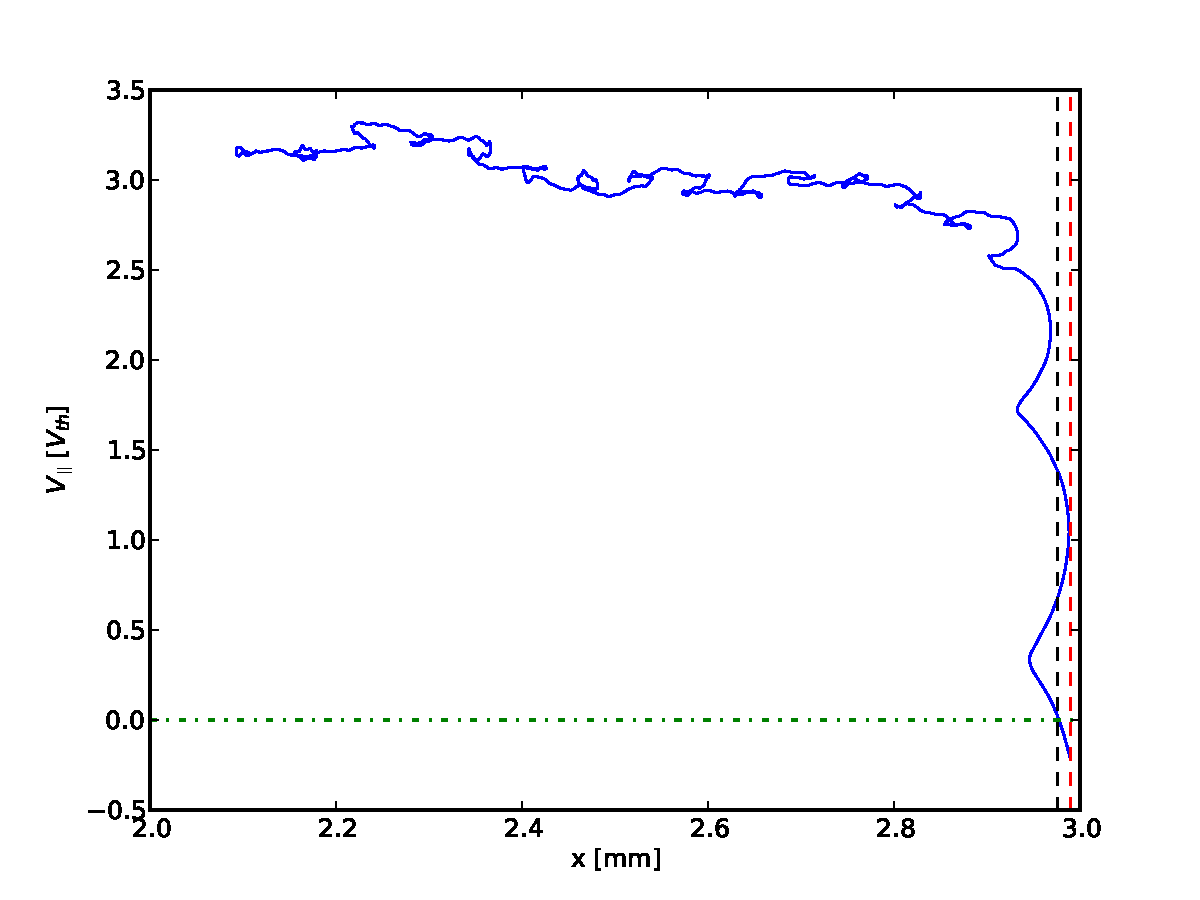
\includegraphics[width=0.9\textwidth]{absorbed_negative_electron.pdf}
	\caption{A plot of the parallel velocity of an electron that reaches the probe due to finite orbit effects as it moves through the bulk plasma, into the sheath, before reaching the probe surface. The two vertical dashed lines represent a region of width 1 $\rho_e$ away from the probe. The electrons parallel velocity rapidly drops in the sheath, becoming negative within the marked region. At this point its orbital motion brings it to the probe.}
	\label{fig:absorbed_electron}
\end{figure}



The collection of electrons with a negative parallel velocity was reproducible in 1D3V simulations, allowing for parameter scans to be carried out. These parameter scans varied the ratio $\lambda_D / \rho_e$ to test its effect on the measured electron temperature. The ratio was adjusted by varying either the magnetic field strength or plasma density. In addition to these simulations, a temperature scan was carried out and an angle scan. Presented in figure \ref{fig:relative_error} are the results of the magnetic field and plasma density scans. Increasing the ratio $\lambda_D / \rho_e$, reduces the relative error in the temperature measurement. 

\begin{figure}[H]
	\centering
	\includegraphics[width=0.9\textwidth]{relative_error.pdf}
	\caption{The relative error in the electron temperature measurement ($T_e^{measured} / T_e ^{source}$) as a function of $\lambda_D / \rho_e$. Shown in the dashed lines are approximate values of $\lambda_D / \rho_e$ based on typical divertor conditions for MAST \cite{MAST_DIV}, ITER \cite{ITER} and CMOD \cite{CMOD_DIV}. }
	\label{fig:relative_error}
\end{figure}

The effect also has an angle dependency. For cases where $\theta = 90$, the gyromotion of the electron has no component towards the probe and so this effect is not present. As the angle becomes more shallow, the relative error increases. The relative error in the temperature measurement as a function of angle is shown in figure \ref{fig:angle_error}. The relative error was fitted to a function  $h(\cos\theta / \sqrt{\sin\theta})+1$, where $h$ is a constant. The $\cos \theta$ term represents the component of the electrons gyroradius directed normal to the probe surface, while the $\sqrt{\sin \theta}$ term takes into account the increase in the local Debye length due to the MPS density drop. At a density of $6.4 \, \times \, 10^{18} \, m^{-3}$, a field strength of $0.4$ T and a temperature for both species of $6$ eV, it was found that $h = 0.055$. This value may change for different plasma parameters. This result provides further evidence that the ratio $\rho_e / \lambda_D$ plays a key role in the error of the temperature measurement.


Simulations were carried out varying the electron temperature whilst keeping the magnetic field strength and plasma density constant. For the case described above, with a density of $ 6.4 \, \times \, 10^{18} \, m^{-3}$ and a magnetic field strength of $0.4$ T at an angle of $12^{\circ}$, the relative error in the temperature measurement was $\approx 10\%$ for a range of specified $T_e$ from $6 \to 48$ eV. Both $\lambda_D$ and $\rho_e$ have a $\sqrt{T_e}$ dependency so the ratio of $\lambda_D / \rho_e$ remains constant as $T_e$ is varied.

\begin{figure}[H]
	\centering
	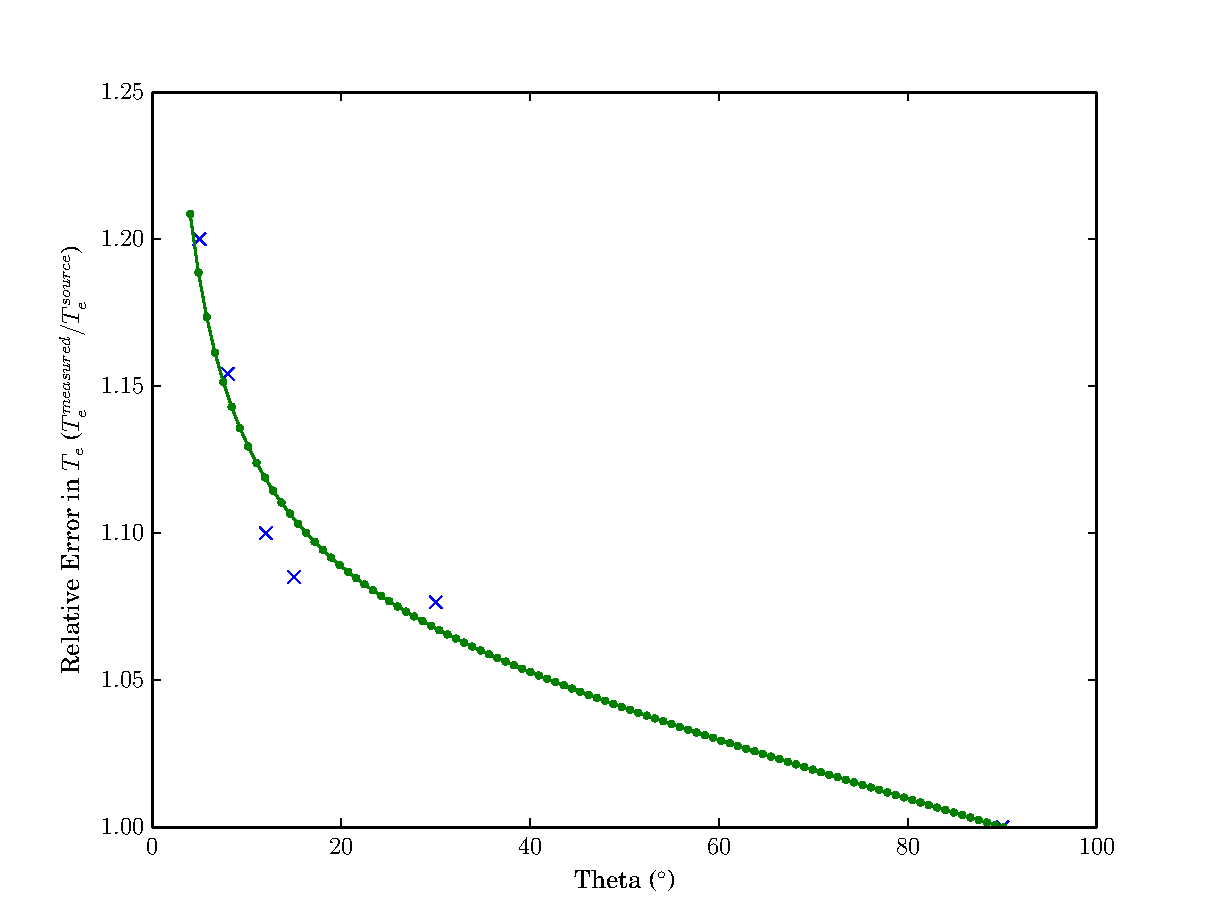
\includegraphics[width=0.9\textwidth]{angle_error.pdf}
	\caption{The relative error in the electron temperature measurement ($T_e^{measured} / T_e ^{source}$) as a function of $\theta$. The green line is a fitted function of the form $h(\cos\theta / \sqrt{\sin\theta})+1$. Where $h$ is a constant. }
	\label{fig:angle_error}
\end{figure}
In future machines, the high density and low angle of attack necessary for divertor tiles to survive the high heat loads, will place FMPs on these devices on the LHS of figures \ref{fig:relative_error} and \ref{fig:angle_error}. Although this will somewhat be compensated by stronger magnetic fields, a complete theory to take into account the finite electron Larmor radius effect is necessary to reduce the error in $T_e$ measurements.  This theory is complicated as it depends on both $\rho_e$ and $\lambda_D$  both of which depend on $T_e$ and the latter also depends on $n_e$. These are the two quantities the probe is trying to measure.





\section{Analysing Experimental Data} 
In this section both the no-gap model \cite{Bergmann-2002} and the gap model are fitted to experimental data obtained from a FMP on MAST and the results obtained are compared to the standard fitting procedure. The shot number was 30356. The data was analysed at time $t = 0.315818$ s, with a  toroidal field strength $B_t = 0.369$ T. The magnetic field made an angle $\theta = 8.46 ^\circ$ with the probe surface. 
In the standard fitting procedure, first a straight line is fitted to the ion saturation region to give an estimate of $I_{sat}^+$. This method does not take into account sheath expansion effects. Once a value for $I_{sat}^+$ has been obtained this value is fixed and the following function is then fitted to the I-V curve up to the floating potential
\be
I = I_{sat}^+\left(1 - \exp\left(-\frac{V_{f,fit} -V_{probe}}{T_{e,fit}}\right)\right)
\ee 
Here $V_{f,fit}$ and $T_{e,fit}$ are free parameters. The values obtained for the two variables are then used as initial guesses along with $I_{sat}^+$ for fitting to the I-V curve with all three variables now free parameters. This returned the following values $I_{sat}^+ = 0.0316$ A and $T_e = 9.97$ eV. The density is related to the saturation current by the following equation 
\be 
n_e = \frac{I_{sat}^+}{c_s A_{probe} q\sin\theta} 
\ee
In the standard fitting procedure it is assumed that the sound speed is given by 
\be 
c_s = \sqrt{T_e q/m_i}
\ee  
The fitted values then give a density $n_e = 4.34 \times \, 10^{18}$ $m^{-3}$. However, from the FMP simulations, the sound speed is better described by $c_s = \sqrt{(T_e + \gamma_i T_i)/m_i}$ where $\gamma_i = 2$ for low angles of incidence. Using this new value and assuming $T_e = T_i$ gives a lower density of $ 2.51 \times \, 10^{18}$ $m^{-3}$. 
Now applying the no-gap model to the data. Firstly a function is fitted to the ion saturation region, in this region it is assumed the electron current is zero, the current to the probe is then described by 
\be 
I = I_0 \left( 1 + a {\left(\frac{V_f - V_{probe}}{T_e}\right)}^{3/4} \right)
\ee
$T_e$ and $V_f$ are taken from the standard fitting procedure. This returns a value for $I_0$ and $a$. The latter two variables are then fixed and a fit to the I-V curve up to the floating potential is carried out to get a new estimate for $T_e$ using the following function 
\be 
I = I_0 \left( 1 + a {\left(\frac{V_f - V_{probe}}{T_{e,fit}}\right)}^{3/4}  - \exp\left(-\frac{V_f-V_{probe}}{T_{e,fit}}\right) \right)
\ee 
As before, the values of $I_0$ and $T_e$ are used to obtain an initial estimate for $n_e$. A full fit is then carried out using the obtained values as initial estimates. Both $I_0$ and $a$ themselves depend on $T_e$ and $n_e$. $I_0$ is proportional to the density and depends on temperature through the sound speed. $a$ is proportional to the Debye length.  The full fit equation is then given by 
%\be 
%q n_{e,fit} A_{probe} \sin\theta \sqrt{3T_{e,fit}q/m_i} \left( 1 + \frac{0.5+0.6 \cot\theta}{L\sin^{1/2} \theta} \sqrt{\frac{\epsilon_0 T_{e,fit}}{n_{e,fit} q}}      {\left(\frac{V_f - V_{probe}}{T_{e,fit}}\right)}^{3/4}  - \exp\left(-\frac{V_f-V_{probe}}{T_{e,fit}} \right)\right)
%\ee


\be 
A n_{e,fit}  \sqrt{T_{e,fit}} \left( 1 +  B \sqrt{\frac{ T_{e,fit}}{n_{e,fit}}}      {\left(\frac{V_f - V_{probe}}{T_{e,fit}}\right)}^{3/4}  - \exp\left(-\frac{V_f-V_{probe}}{T_{e,fit}} \right)\right)
\ee
where $A$ and $B$ contain the constants of the fit.
\be 
 A = \sqrt{3/m_i} q^{3/2} A_{probe} \sin\theta
\ee 
\be 
B = \frac{0.5+0.6 \cot\theta}{L\sin^{1/2} \theta} \sqrt{\frac{\epsilon_0}{q}}
\ee

% *  ( (0.5 + 0.6 / tant)*sqrt(deb_con*te_fit/ne_fit)/(5e-3*sqrt(sint)) * ((vf-x)/te_fit)**0.75 + 1 -1*np.exp(-1*((vf-x)/te_fit)))
The density and temperature estimated from the standard fit give rise to a Debye length such that $L/\Lambda_D \approx 420$. It is then valid to take $c_2 = 0.6$. In lower density cases $c_2$ would have to be treated as a free parameter.
Applying this fit gives $n_e = 2.26 \times \, 10^{18}$ $m^{-3}$ and $T_e = 9.21$ eV. So both quantities have decreased now that sheath expansion has been taken into account. To take into account the presence of the 1 mm gap in between the wall and the probe, three adjustments must be made. Firstly, $A_{probe}$ increases from $2 mm \times 5 mm$ to $(2 mm \times 5 mm) + (1 mm \times 2mm) $ to take into account the exposed area of the side. $L$ in the $B$ coefficient is replaced by ($L + 1$ mm) and finally, the value of $c_1$ is increased to 0.9. Applying this new fit to the data gives $n_e = 1.88 \times \, 10^{18}$ $m^{-3}$ and $T_e = 9.22$ eV. The density is a $20 \%$ reduction on that as measured by the no-gap model whilst the electron temperature is the same. Densities on MAST are typically quoted with error bars of around $1 \%$. The failure to take into account the gap is then a significant source of error. The fits to the data are shown in figure \ref{fig:data_fit}. The no-gap model and gap model provide an almost identical fit to the data, the interpretation of the fitted values is the distinguishing factor.

\begin{figure}[H]
\centering
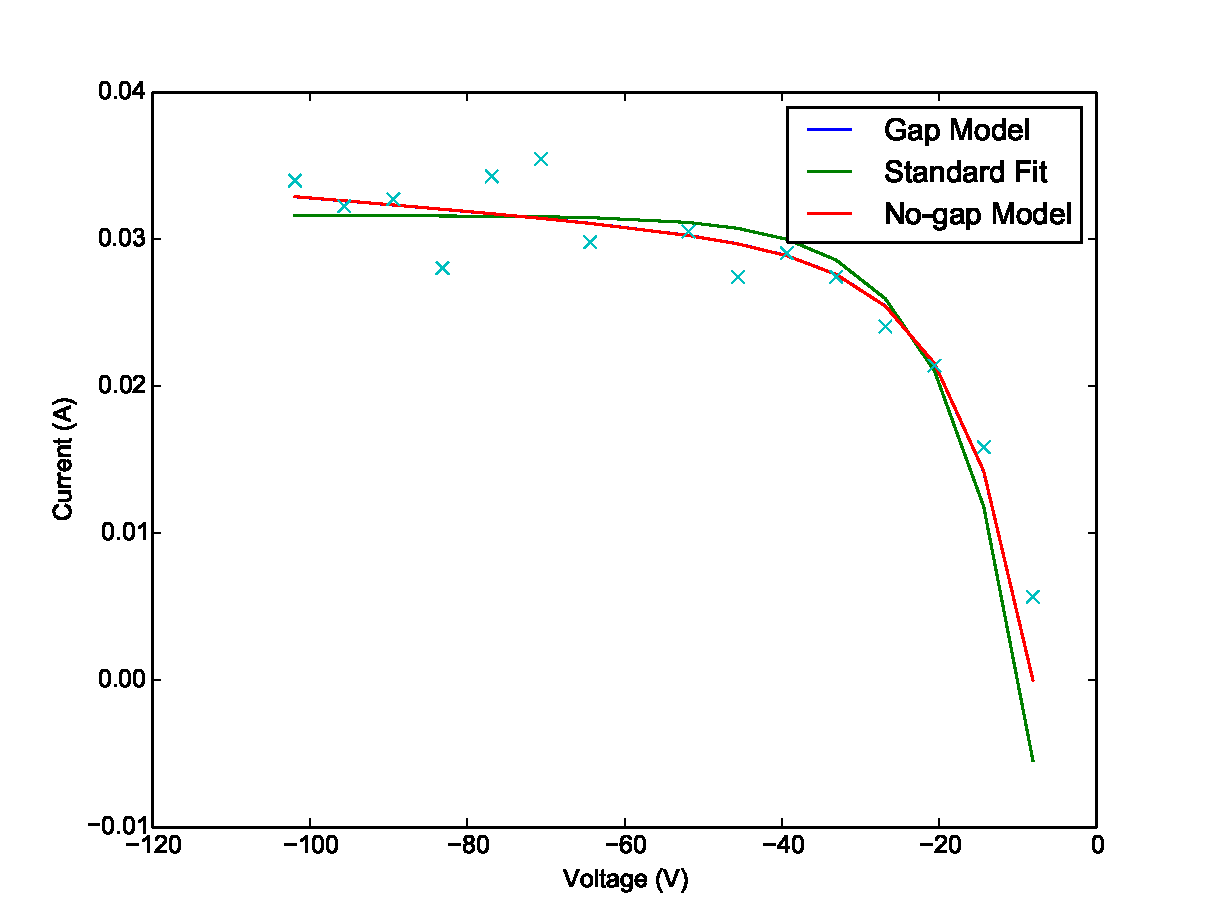
\includegraphics[width=0.9\textwidth]{all_fits.pdf}
\caption{Fits to the MAST data for the three models.}
\label{fig:data_fit}
\end{figure}

Based on the density and temperature values derived from the gap model, the ratio of $\frac{\lambda_D}{\rho_e}$ = $0.8$. A very approximate overestimation of the temperature of $10\%$ could be expected.


%Bergmann gets 2.25939074e+18   9.20530507e+00 so both have decreased slightly 

%Use  bergmanns model c1 = 0.5 c2 = 0.6  

%THen fit line with slope to Isat region to allow for sheath expansion, assuming Te and Vf found from basic fit are correct. This gives I0 and 'a'


%new cs and gap main effects 
%
%LD = 1.5e-5  
%RL = 2 e-5 
%Ratio 0.75 so temperature etimated may be too high by approx 10 percent

%Fix that I0 value and a  fit curve  up to floating potential to get a new estimate for Te  


%use Te estimate to get estimate for Cs. Use Cs estimate to get estimate for density. Then full fit using these initial guesses 


%If not dense enough then c2 would have to be a free parameter


%WIth my model change c1 value but not area first of all, what effect does that have?  Then change area but not c1 then both. 
%
%On changing c1 value My FUlly fit values [  2.25558604e+18   8.99940561e+00]
%slight decrease in density reduction in temp  
%
%Then changing the area and the d+g bit in 'a'
%1.88307217e+18   9.22083625e+00
%
%Densities on MAST usually quoted with errors +/- 1%,
%Failing to take into account the gap produces a 20% error 
%roughly estimate error in Te













%Shot # 30356
%t = 0.315818
%mux 4
%probe 7
%Bt = 0.369 T
%theta = 8.46 deg
%Te = 8 +/- 0.7 eV
%ne = 2.84e18 +/- 2.7e16

%$basic fit  $
%Fit straight line to Isat region 
%
%Then fit following fucntion keeping Isat fixed to whole IV curve 
%$isat*( 1- np.exp((-1*(v_ffit-x)/TE_fit)))$
%
%Then have all of them as free variables using those values as initial guesses  fititng up to floating potential
%$ne = 4.34374144337e+18$
%
%$assumed te = ti and cs = cs = sqrt(te*1.6e-19/(m_i)) $
%Te = 9.9 eV 
%$new ne with new cs =  2.50786029162e+18$
%







\section{Discussion}
The simulations of \cite{Bergmann-2002} have been reproduced in VSim and extended to incorporate a gap in between the probe and the floating divertor tiles. This gap is present in all machines and is especially important for the FMPs on MAST as the gap size is significant compared to the length of the probe. The presence of the gap was found to enhance the effective collection area of the probe and therefore needs to be included in probe data interpretation in order to extract the correct plasma density from the I-V characteristics. Non-saturation of the ion current was also observed in the gap simulations. The sheath expansion parameter $a$ is slightly reduced from the no-gap model. The predominant effect on experimental data interpretation is the enhancement of the effective collection area of the probe. For MAST probes, the density is overestimated by $20\%$ if the gap is not included. 

Full resolution of the electrons gyromotion reveals a portion of the electron current to the probe consists of electrons with insufficient parallel energy to overcome the sheath potential. These electrons are able to reach within a Larmor orbit of the probe and are then reflected away from the probe. At this distance from the probe surface, their motion around the magnetic field is able to bring them to the probe. This effects all regions of the I-V characteristic in which the probe is biased below the plasma potential. Applying standard probe theory to the electron current in simulations where the magnetic field makes a shallow angle to the probe surface, produces measurements of the electron temperature that are too high. If the correct electron temperature is to be extracted from probe I-V curves, a theory is required that takes into account the additional current to the probe that consists of electrons reaching the probe due to their orbit.
The use of strong magnetic fields will reduce the effects of sheath expansion and the finite electron gyro-orbit. For strong magnetic fields the ions remain tied to magnetic field lines, even in the Debye sheath and so the probe collects current over its projected length ($(L+g)\sin\theta$). The Larmor orbit of the electrons is reduced too so less electrons are capable of reaching the probe without having sufficient parallel energy to overcome the sheath potential.

It would be useful to extend this work to smaller magnetic field angles as future machines will aim to reduce $\theta$ to the minimum of engineering limits, to minimise the thermal load on the diveror components. In \cite{Bergmann-2002}, the influence of E x B drifts on particle collection by FMPs was investigated. The drifts caused an enhancement of the ion current to the probe but this effect was much smaller than the ion focusing effect. A reduction in the electron current was observed for a probe biased near the plasma potential. These effects indicate that  three-dimensional PIC simulations of the FMPs would be beneficial to allow further investigation into the charged particle collection of these probes. Due to Debye lengths on the order of $\mu$m and probe lengths on the order of mm, three-dimensional PIC simulations are extremely computationally intensive.

%Future work extending to smaller angles, 3d ims 


%Talk about extent of sheath magnetisation from Gunns paper In very strong fields, sheath effects and electron temp problems go away

%Extending to smaller angles for other machines

%Limitations of 2D model, ExB drift direction neglected, what did Bergmann find on this in his second paper?


%Assume Ti = Te
%Here we extend upon the detailed work carried out by Bergmann for FMP installed on MAST. As with Bergmann's simulations, realistic probe length to ion gyroradius ratios are used in the simulations. In these simulations, a gap between the FMP and the wall is included to better replicate the experimental set-up. The effects of the gap on the sheath expansion parameter are explored. The presence of the gap is found to reduce the sheath expansion parameter but this is a minor effect. The electrons in Bergmann's simulations were treated in guiding-centre approximation \cite{Bergmann-1994} however, in our simulations, both electrons and ions are treated kinetically and the complete motion of both species is resolved fully. An important effect has been observed as a result of this treatment. A significant portion of the electron current to the probe, at any negative bias voltage, is made up of electrons whose energy parallel to the field is not sufficient to overcome the probe sheath potential. These electrons are able to propagate through the sheath to within an electron gyroradius ($\rho_e$) before reflecting away from the probe. At this point their orbit around the field is able to bring them to the probe. This effect increases the derived temperature from the simulated FMP if not accounted for. 

%Reported here are results from two and three-dimensional PIC simulations using VSim \cite{VORPAL}. Section X details the simulation model. In section X the effect of the gap on FMP ion collection is explored. Electron collection by FMP is explored in section X and results from three-dimensional simulations are presented in section X.  




\section{References}
\bibliography{references}
	
\end{document} 
